
% VLDB template version of 2020-08-03 enhances the ACM template, version 1.7.0:
% https://www.acm.org/publications/proceedings-template
% The ACM Latex guide provides further information about the ACM template




\documentclass[sigconf, nonacm]{acmart}
\usepackage{soul}


\usepackage[demo]{graphicx}
\usepackage{subcaption}

%% The following content must be adapted for the final version
% paper-specific
\newcommand\vldbdoi{XX.XX/XXX.XX}
\newcommand\vldbpages{XXX-XXX}
% issue-specific
\newcommand\vldbvolume{14}
\newcommand\vldbissue{1}
\newcommand\vldbyear{2020}
% should be fine as it is
\newcommand\vldbauthors{\authors}
\newcommand\vldbtitle{\shorttitle} 
% leave empty if no availability url should be set
\newcommand\vldbavailabilityurl{URL_TO_YOUR_ARTIFACTS}
% whether page numbers should be shown or not, use 'plain' for review versions, 'empty' for camera ready
\newcommand\vldbpagestyle{plain} 

\begin{document}
\title{Green Investing using Alternative Data Sources}

%%
%% The "author" command and its associated commands are used to define the authors and their affiliations.
\author{Kamila Zaman}
\affiliation{%
  \institution{New York University}
}
\email{kz2137@nyu.edu}

\author{Jorge Roldan-Roldan}
\orcid{0000-0002-1825-0097}
\affiliation{%
  \institution{New York University}
}
\email{jlr9718@nyu.edu}

\author{Antony Sunwoo}
\orcid{0000-0001-5109-3700}
\affiliation{%
  \institution{New York University}
}
\email{as10506@nyu.edu}

%%
%% The abstract is a short summary of the work to be presented in the
%% article.
\begin{abstract} Data driven decision making is key to success. Living in this age of Big Data with numerous cutting edge technologies we have great opportunities at our disposal to make use of these resources to drive this data driven decision making approach into a reality and a culture for the current and upcoming industries. The rising global concern regarding climate change and the catastrophes it most probably might lead up to has given rise to several new companies being formed, organizations establishing new short-term/long-term policies and agreements;signed and presented to mange this issue with increased importance and priority. This mounting awareness is the cause for establishment of many new companies jumping into this industry along with the older ones improving, revamping and aligning their goals in agreement with climate change concerns as well. This gives us the perfectly timed opportunity to dive into putting forth an idea and methodology to explore the predictive power of the data for investment opportunities in this upcoming industry of Green Energy Companies based on understanding at greater depths driven with creativity to analyse, comprehend and formulate an approach applicable to see forthcoming stock-trend's for individual companies and as whole groups to facilitate investors before hand to maximize developments and profits an make the companies with a good cause to grow further. 
\hl{done by me- change anything you feel doesnt fit}

%In this project we explore the use of Twitter and News article as alternative data sources to predict the stock values of green companies such as First Solar, Siemens, etc. 
\end{abstract}

\maketitle


% %%% do not modify the following VLDB block %%
% %%% VLDB block start %%%
% \pagestyle{\vldbpagestyle}
% \begingroup\small\noindent\raggedright\textbf{PVLDB Reference Format:}\\
% \vldbauthors. \vldbtitle. PVLDB, \vldbvolume(\vldbissue): \vldbpages, \vldbyear.\\
% \href{https://doi.org/\vldbdoi}{doi:\vldbdoi}
% \endgroup
% \begingroup
% \renewcommand\thefootnote{}\footnote{\noindent
% This work is licensed under the Creative Commons BY-NC-ND 4.0 International License. Visit \url{https://creativecommons.org/licenses/by-nc-nd/4.0/} to view a copy of this license. For any use beyond those covered by this license, obtain permission by emailing \href{mailto:info@vldb.org}{info@vldb.org}. Copyright is held by the owner/author(s). Publication rights licensed to the VLDB Endowment. \\
% \raggedright Proceedings of the VLDB Endowment, Vol. \vldbvolume, No. \vldbissue\ %
% ISSN 2150-8097. \\
% \href{https://doi.org/\vldbdoi}{doi:\vldbdoi} \\
% }\addtocounter{footnote}{-1}\endgroup
% %%% VLDB block end %%%

% %%% do not modify the following VLDB block %%
% %%% VLDB block start %%%
% \ifdefempty{\vldbavailabilityurl}{}{
% \vspace{.3cm}
% \begingroup\small\noindent\raggedright\textbf{PVLDB Artifact Availability:}\\
% The source code, data, and/or other artifacts have been made available at \url{\vldbavailabilityurl}.
% \endgroup
% }
% %%% VLDB block end %%%


% % ========================================================
% % ========================================================
% \section{Professor Instructions}
% % ========================================================
% % ========================================================
% \hl{
% The project report should include an abstract, introduction and a literature review on related works and papers on your project. Then the following sections should follow the CRISP-DM: Data understanding (describe your data, data sources, relevance to your project), Business Understanding (problem statement, how your approach relates to solving a problem or experimenting a hypothesis...), Data Preparation (algorithms, data reduction, ....), Modeling, Evaluation and Deployment (if applicable..) }

% ========================================================
% ========================================================
\section{Introduction}
% ========================================================
% ========================================================
\hl{Must finish - END}

% ========================================================
% ========================================================
\section{Literature Review}
% ========================================================
% ========================================================
The usage of alternative data sources such as Twitter feeds, news articles and search queries for predicting financial markets has been increasingly receiving attention in industry and academia. The authors in \cite{DBLP:journals/corr/abs-1010-3003} have used used Twitter feeds to investigate the correlation between the public mood and the value of the Dow Jones Industrial average. They used Opinion Finder (OF) and Google-Profile of Mood States (GPOMS) to track the sentiment mood collective mood. The authors also used a Granger causality analysis and Self-Organizing Fuzzy Neural Network to determine whether the collective mood is indeed correlated to the values of the DJIA, and successfully found an accuracy of 87.6 percent in predicting the daily behavior  of this index. \\
Authors in \cite{8713246} have used news articles besides Twitter feeds as an additional alternative data source. The authors used Opinion Finder (OF) and Stanford Natural Language Processing Programming Interface (SNLP) to do the sentiment analysis of these sources. Furthermore, they adopted a  Time-based Term Frequency and Inverse Document Frequency (TF-IDF) to  normalize the frequency of terms and used it to cluster terms using clustering algorithms. In this work the authors also dr
d correlation analysis and Granger causality as well as other linear regression models to study the correlation between the collective mood from these data sources and the stock market behavior of various entities in Australia. 

% ========================================================
\section{Business Understanding}
% ========================================================
\hl{Must finish - Understanding the stock market and terminologies, and unders}

% -------------------------------------------------------
\subsection{Background}
% -------------------------------------------------------
\begin{flushleft}
It is now evident, as it has been for a long time that we are facing a climate crisis and there is not question about the urgent need to take action on this crisis. The Intergovernmental Panel On Climate Change has stated that Scientific evidence for warming on the climate system is unequivocal and that there is a 95\% probability to be the result of human activity \cite{nasa_2021}.  Some of evidence that confirms this crisis is the increase of 2.12 degrees Fahrenheit  of the planet's average surface temperature, the warming of the ocean of more than 0.6 degrees Fahrenheit, the average lost of 279, and 148 billion tons of ice per year on Greenland and the Antarctica, respectively. Other evidence include the rise of global sea levels of about 8 inches during the last century, and many other  \cite{nasa_2021}.
\end{flushleft}

\begin{flushleft}
One would think that it is evident the urgent need to invest on green and climate friendly companies and industries, but we live in a country and a world where the influence and interests of some corporations on our government and policy making drastically affect our ability to invest on sectors of the industry which could positively impact our chances to successfully fight against climate change. Now more than ever it is crucial for the global economy to transition to climate friendly industries, and it is paramount for the biggest economies such as the US to play a key role in this transition. 
\end{flushleft}


% --------------------------------------------------------
\subsection{Stock Market Understanding}
% --------------------------------------------------------
Our attempt to investigate the stock market behaviour naturally requires a 
    ETF Terms 
Tickers - Public Companies
Clean energy indices - S\&P clean energy index

\hl{Must finish}
% --------------------------------------------------------
\subsection{Clean and Green Energy Industry }
% --------------------------------------------------------
Top Green Energy company - survey
Major events or global concern regarding clean energy
Some major issues gaining attention:
Warming of the ocean of more than 0.6 degrees Fahrenheit
Increase of 2.12 degrees Fahrenheit of the planet’s average surface temperature.
Average lost of 279, and 148 billion tons of ice per year on Greenland and the Antarctica, respectively

\textbf{Market Leaders }
\begin{enumerate}
    \item First Solar
    \item Siemens Gamesa
    \item Sunrun
    \item Plug Power
    \item Sun power 
    \item Enphase 
    \item Merdian 
\end{enumerate}





% ========================================================
\section{Data Understanding}
% ========================================================
\hl{highlight}

Data Understanding phase of CRISP- DM Framework focus on collecting the data, describing and exploring the data.
This stage comprises of four key steps to understand the available data, and identify new relevant data in order to solve the business problem. 




% --------------------------------------------------------
\subsection{Collection of Initial Data} % initial data collection report
% --------------------------------------------------------
For this project, we collected three sets of data.

\subsubsection{Twitter Data}
The Twitter Data was obtained from the official Twitter API. We were able to obtain an Academic License which allows us to collect up to 10 million tweets per month. For our purposes, we collected around 1 million tweets for the 7 companies identified in the business understanding phase from 2011 to 2020 using the full archive end point. With the streaming API, we also collected around 1500 tweets for each company daily.

\subsubsection{News Article Data}
The News article data was collected using Bing News Search API. We used the Basic License, which gave 1000 requests per month. Each request gave up to 100 news articles, which could include duplicates from previous queries. The API also only retains articles up to one month old. This was naturally very limited. We were able to collect around 200 unique news articles per company for one month.

\subsubsection{Stock Prices Data}
To collect the stock price data, we used the open-source Alpha Vantage API. It uses a ticker based search, allowing us to look up each company's stock directly. We collected data for each company with the longest duration allowed.
% --------------------------------------------------------
\subsection{Describe Data} % data description report 
% --------------------------------------------------------
\hl{Describe data — for explicit information: Once you have identified the data set, you need to describe its contents and explore insights to better understand the data and its business implications.}

\subsubsection{Twitter Data}
The query returned by the Twitter API is a JSON file. Each object in the file has the following fields:

\begin{enumerate}
    \item Created at
    \item Tweet ID
    \item Author ID
    \item Tweet text
    \item hashtags
    \item \dots
\end{enumerate}

\hl{check for correctness}


\subsubsection{News Article Data}
The query returned by the Bing News Search API is a JSON file. It included a description of the search, and the list of articles returned by the query. Every article returned have the following fields:

\begin{enumerate}
    \item Item type
    \item Date published
    \item Title
    \item Description
    \item Provider
    \item URL
    \item \dots
\end{enumerate}

Not all data fields are always filled in, but the ones listed seem to be consistently available.

\subsubsection{Stock Prices Data}
The stock prices data for a certain company (ticker) given by AlphaVantage API is in the following format:

\begin{enumerate}
    \item Time Stamp
    \item Close value
    \item Open value
    \item High
    \item Low
    \item Volume
\end{enumerate}

The time stamps values are in day, and the other fields are the corresponding values of the company for that day.

\hl{please check for correctness, initial data before cleaning, no derived values.}

% --------------------------------------------------------
\subsection{Exploratory Data Analysis} % data exploration report 
% --------------------------------------------------------
This phase of the project is a critical part of data understanding, it is exploring the data through plotting charts of various kinds with various combinations. Following types of insights can be achieved through plots/graphs. a) Spotting outlier values b)
Observing trends of variables (increasing/decreasing) etc.c) Observing correlation and use fullness of variables  in context and scope of the problem at hand


\subsubsection{Stock prices - EDA}
\textbf{Attributes' Predicting Value Assessment }
As discussed above, from the API we used to collect the stock price provided various attributes regarding each stock which included:
\begin{enumerate}
    \item Closing price
    \item Opening Price
    \item Daily Highest
    \item Daily Lowest
    \item Volume
    \item Delta - derived attribute(|daily high - daily low| )
\end{enumerate}
Out of all these attributes rather than using every single we one separately and then concluding if it is useful or not we on the other hand decided to apply Auto-correlation based analysis for time series which allowed us to approximate the predicting power of each of the given series based on the randomness it comprises of and eliminated the non-useful ones. 
\\Autocorrelation, also known as serial correlation, it is the correlation of a series with a delayed copy of itself as a function of delay. Informally, it is the similarity between observations as a function of the time lag between them and based on the results of this type of computed correlation we are able to approximate the randomness that a particular series comprises and discard it if there it is an underlying characteristic of it made obvious using the results.
\\ To interpret the result, we should know that if the auto-correlation plot lines lie very close to zero then it can be said that the given series corresponding to one any of the attribute under consideration is random and hence not useful for the time series analysis.

\\ Performing this whole process on all of the given attributes we learnt that the delta attribute is pretty useless as seen in figure (x) and out of the rest, all exhibit the same patter =n hence using any one of it will suffice. We chose to use the "closing price" attribute series. 
\begin{figure}[H]
  \centering
  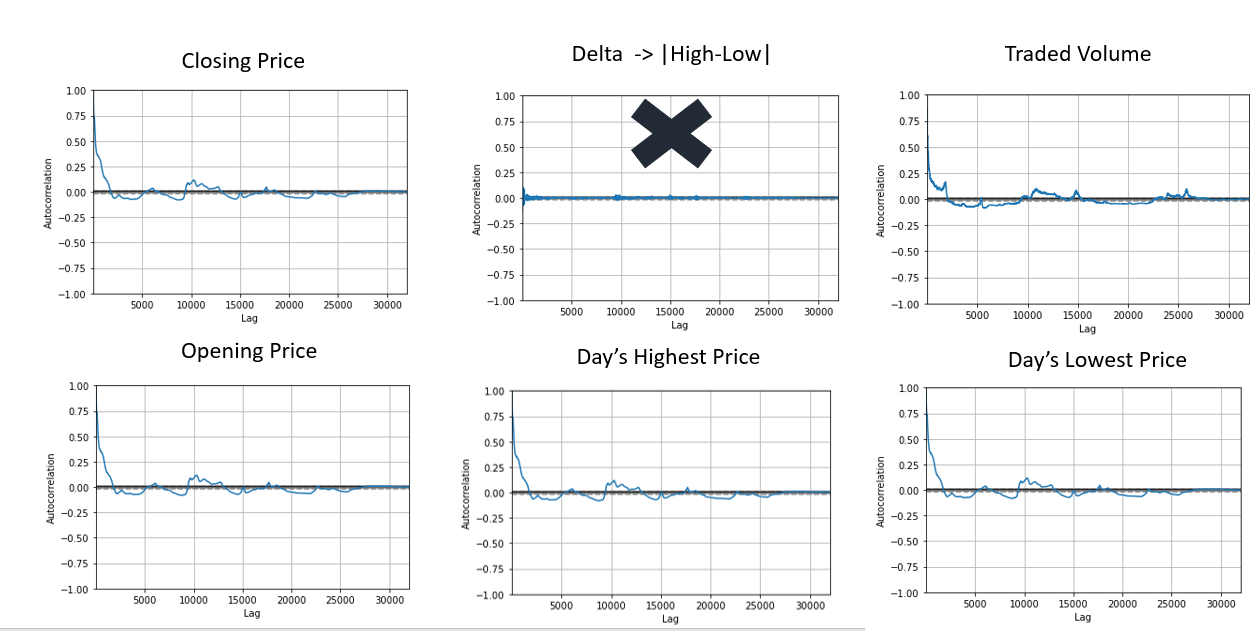
\includegraphics[width=\linewidth]{images/autocorr.PNG}
  \caption{Stock Price Attribute Assessment - Predicting Power/Usefulness for time series Analysis}
%   \label{fig:duck}
\end{figure}



\textbf{Closing Price Trend Plots}
Since we have decided to move forward with the closing price attribute only, we then explored the individual trend lines for the companies under consideration. This plot has two parts where Figure(2) shows the trend of every stocks closing price for the maximum data available and then figure(3) shows the same but a deep dive and closer look at the trend for a single latest year only. The granularity of figure(1) is Yearly quarters where as for the second plot in figure(2) the granularity is of yearly weeks.
\begin{figure}[H]
  \centering
  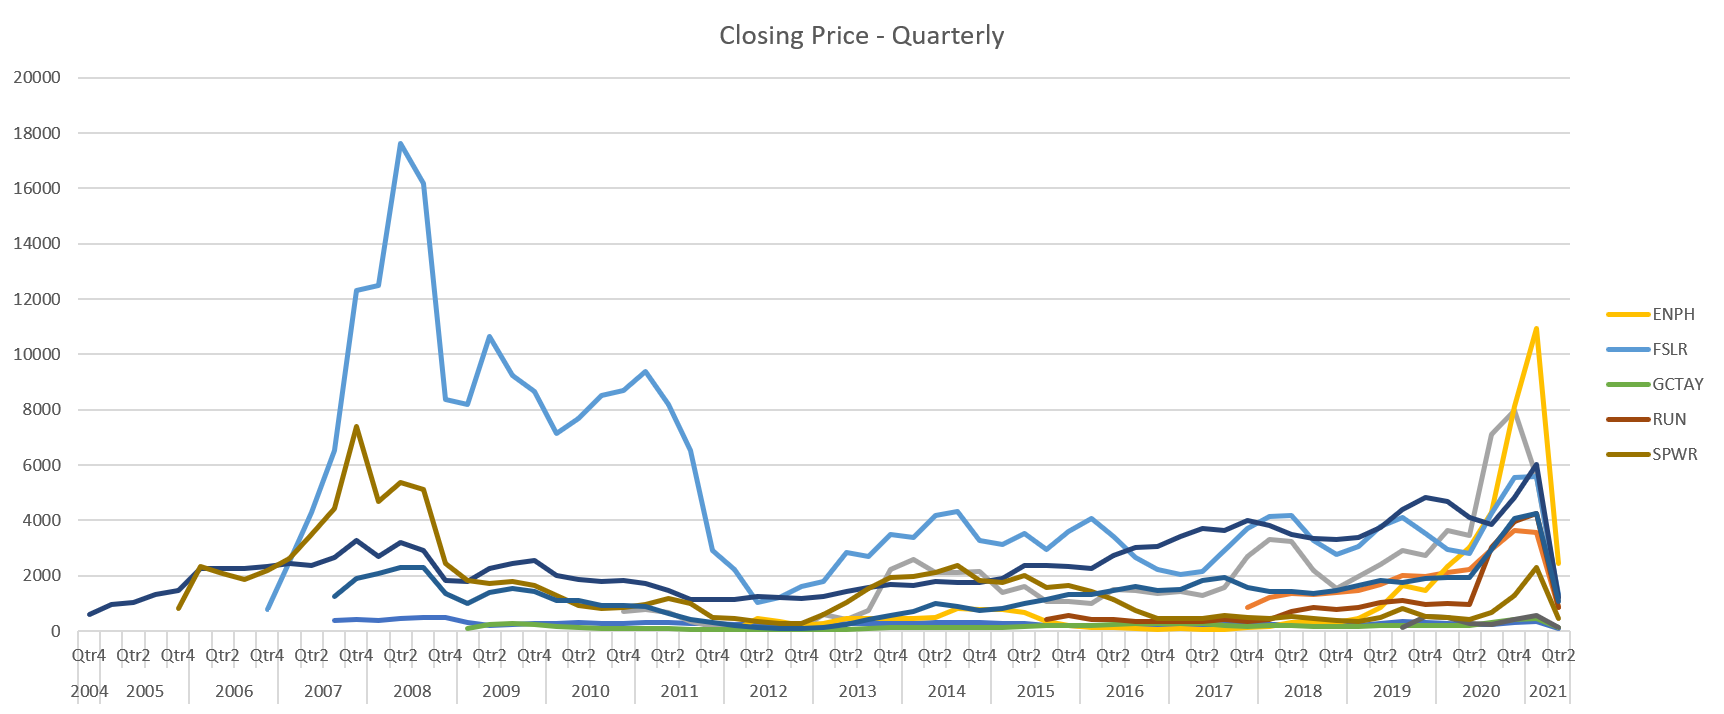
\includegraphics[width=\linewidth]{images/allstocks.png}
  \caption{Stock Prices- Maximum Time Period for every company available}
%   \label{fig:duck}
\end{figure}

\begin{figure}[H]
  \centering
  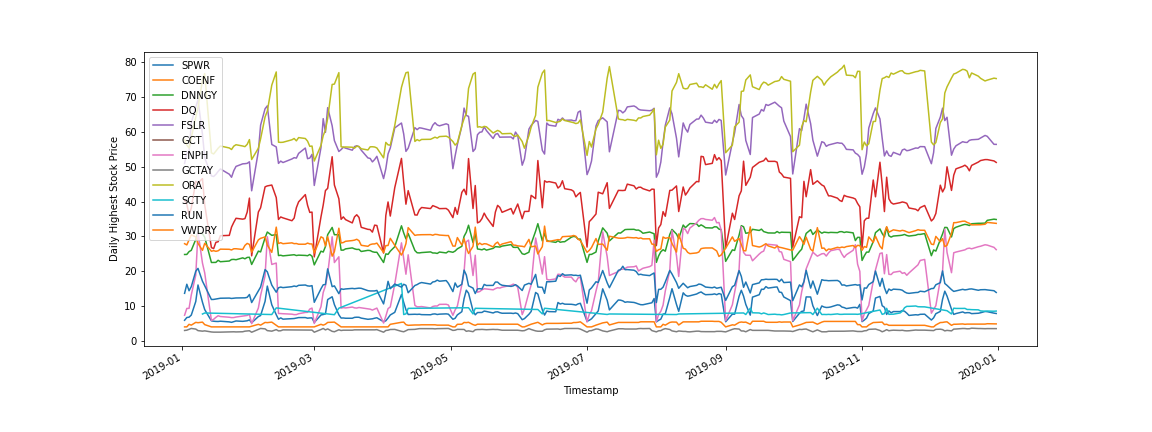
\includegraphics[width=\linewidth]{images/stock_prices_all_2019t20.png}
  \caption{Stock Prices- 2019 - 2020}
%   \label{fig:duck}
\end{figure}




\subsubsection{Twitter Data - Word Clouds}
In the figures(4) and (5) we can see the the word cloud plots for the raw but cleaned twitter data. By raw we mean to specify that it not characterized by sentiment yet rather only split and segregated over individual companies. It was interesting to see what concepts overpowered each of the companies and did actually provide a very good idea of the most important strings attached to each particular company. A good example of it was for siemens where we clearly saw visible focus on solar and wind energy whereas in the remaining one can easily conclude that there wasn't much of he talk around or relevant to wind energy. Another good use of this word-cloud analysis was that is gave us sound basis and reasoning to exclude Tesla's solar power company i.e "Solar City" because one could easily see it being overpowered by Elon Musk related and Tesla related stuff leaving the company itself to be quite insignificant. 
\begin{figure}[H]
  \centering
  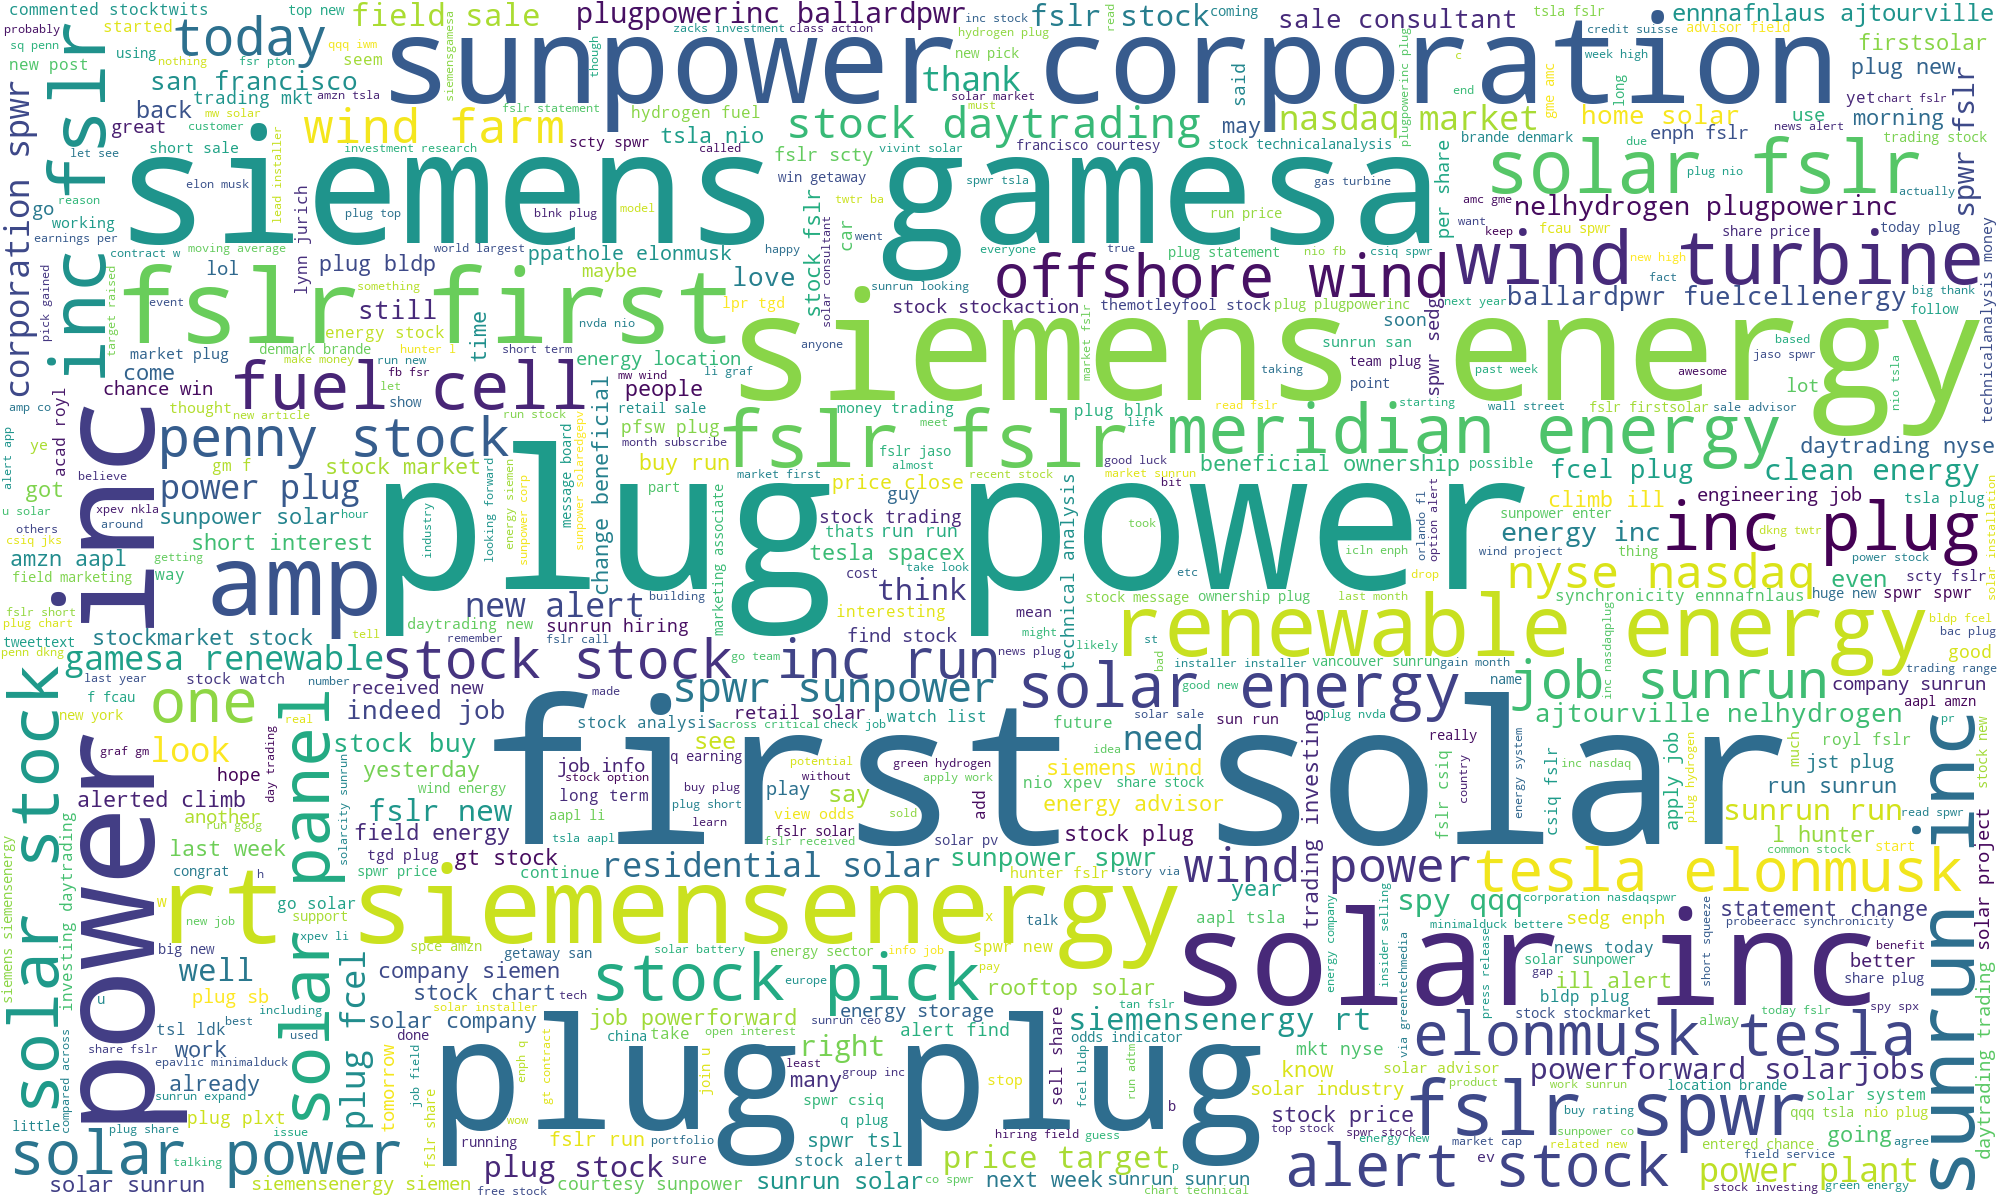
\includegraphics[width=1\linewidth]{images/complete_wordcloud2.png}
  \caption{Word cloud - All Companies Combined}
%   \label{fig:duck}
\end{figure}

\begin{figure}[H]
\begin{subfigure}{0.25\linewidth}
  \centering
  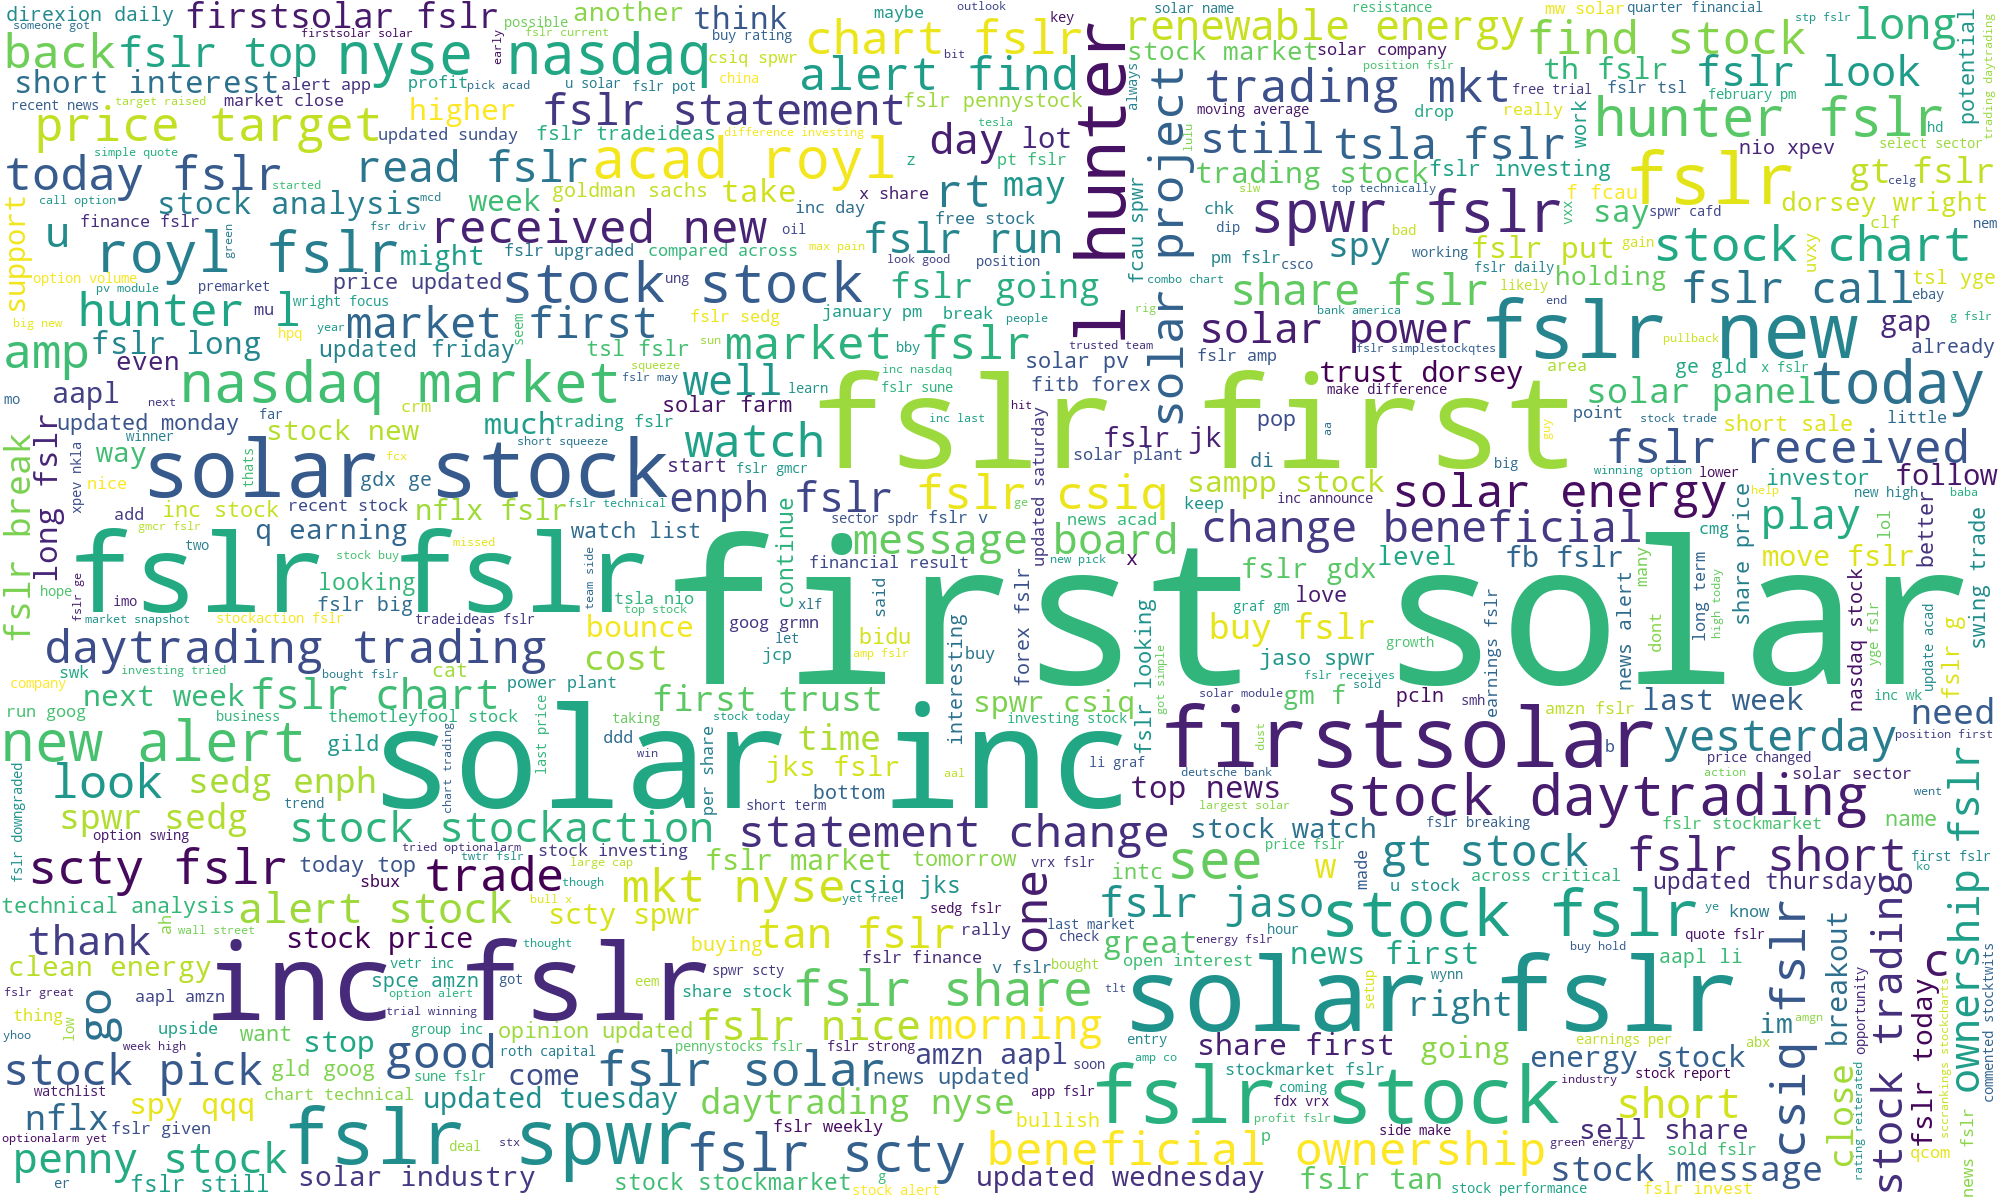
\includegraphics[width=1\linewidth]{images/first_solar_wordcloud.png}
  \caption{First Solar}
  \label{fig:sfig2}
\end{subfigure}%
\begin{subfigure}{0.25\linewidth}
  \centering
  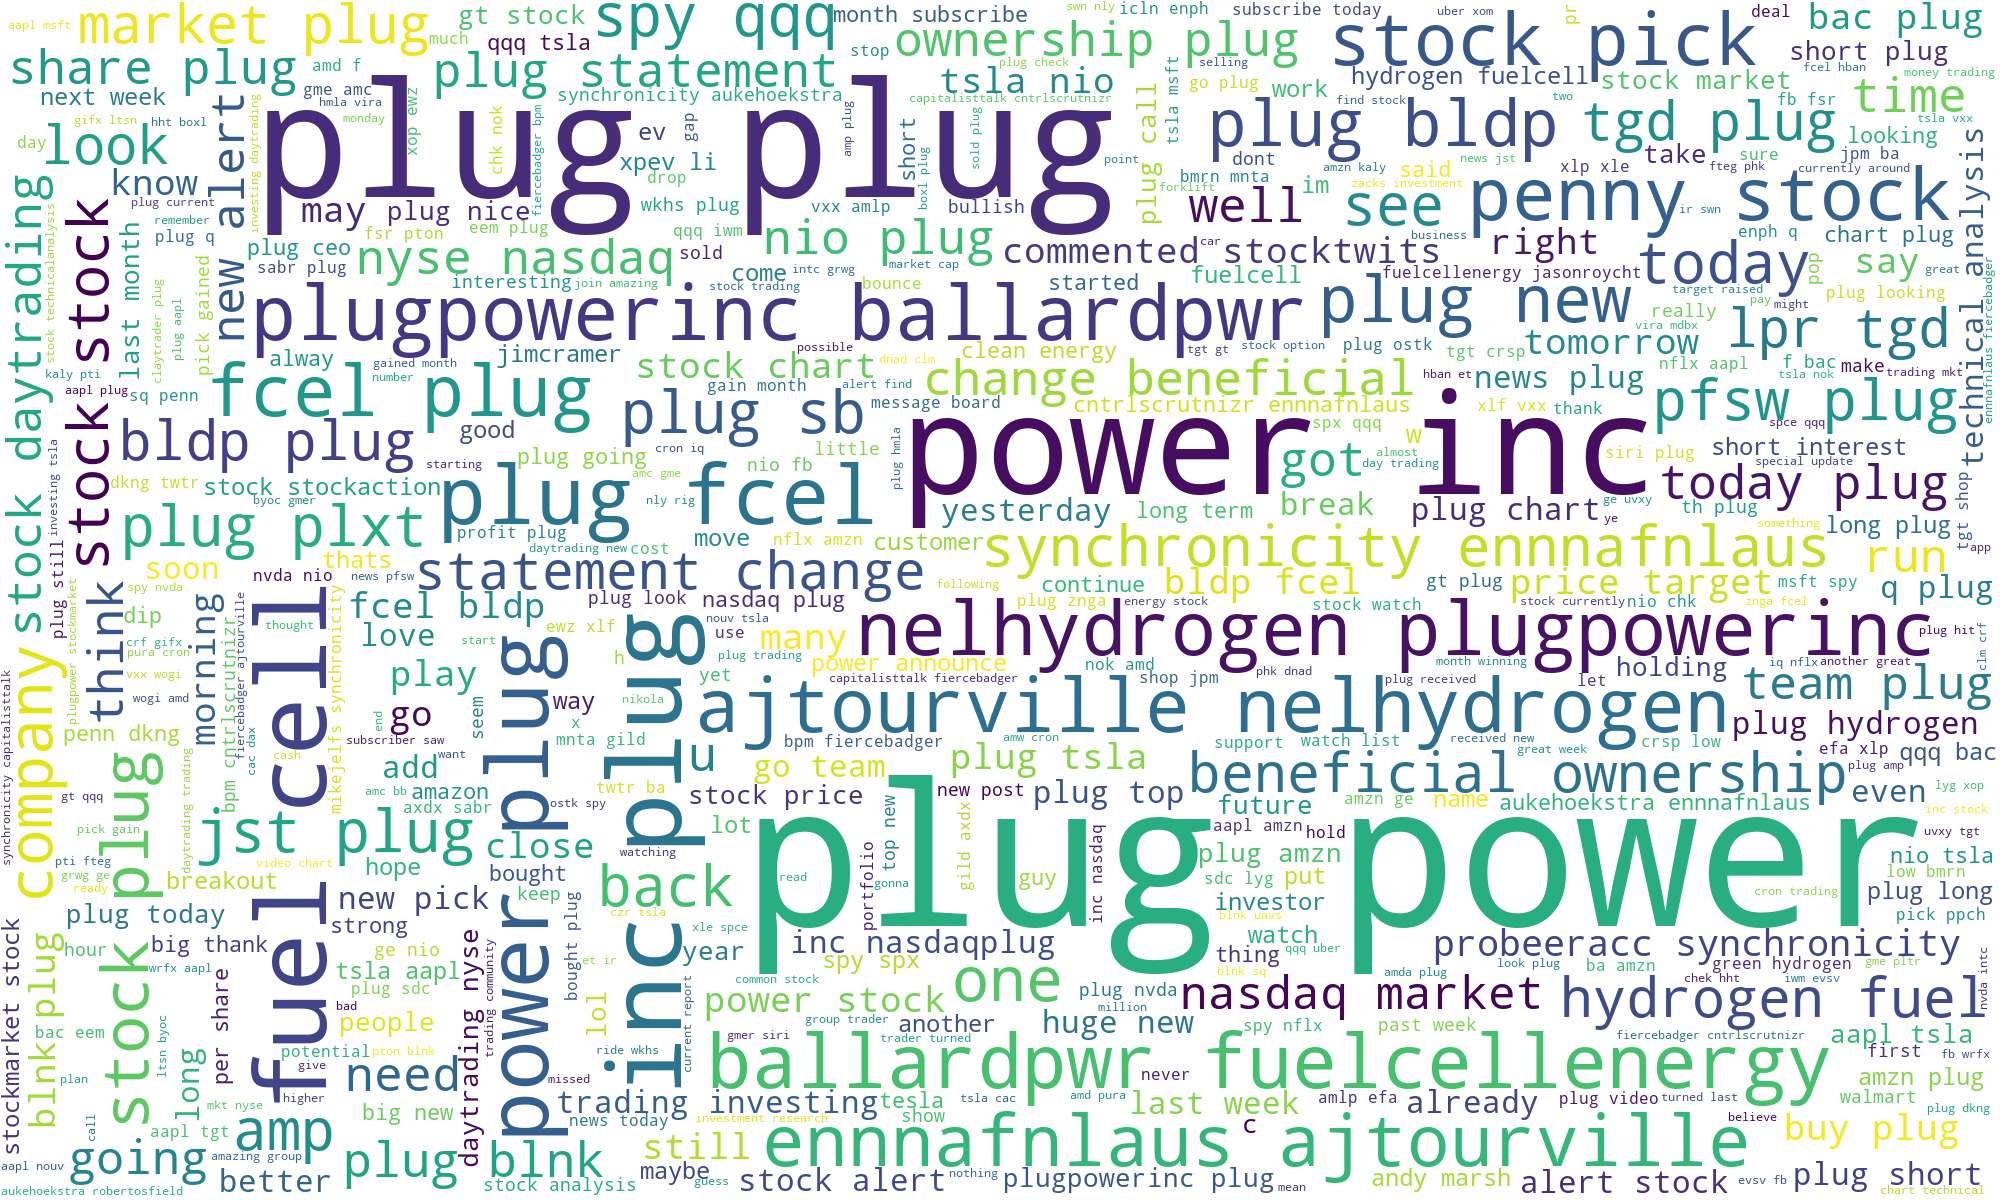
\includegraphics[width=1\linewidth]{images/plug_power_wordcloud.png}
  \caption{Plug Power}
  \label{fig:sfig3}
\end{subfigure}
\begin{subfigure}{0.25\linewidth}
  \centering
  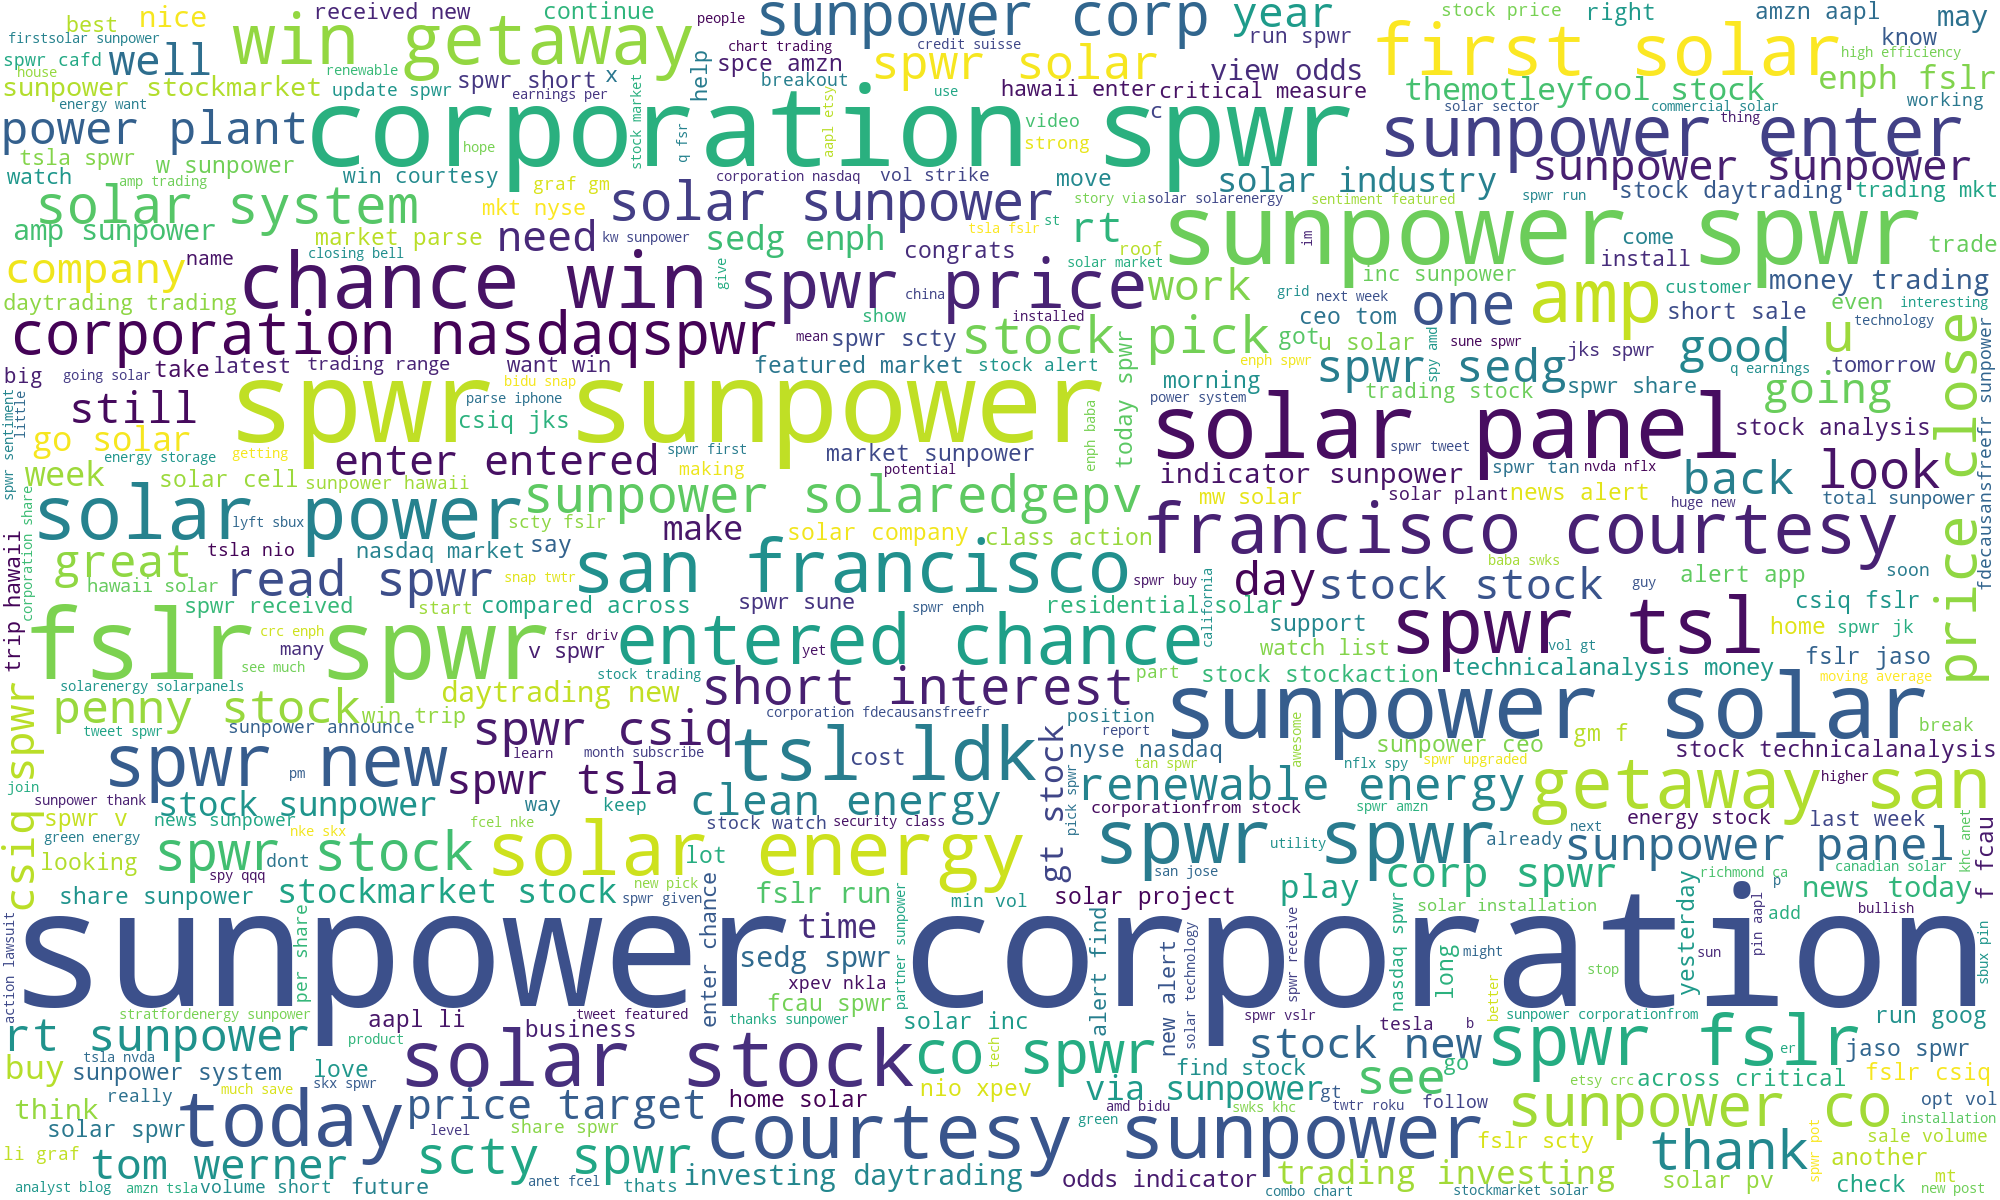
\includegraphics[width=1\linewidth]{images/sunpower_wordcloud.png}
  \caption{Sun Power}
  \label{fig:sfig4}
\end{subfigure}
\begin{subfigure}{0.25\linewidth}
  \centering
  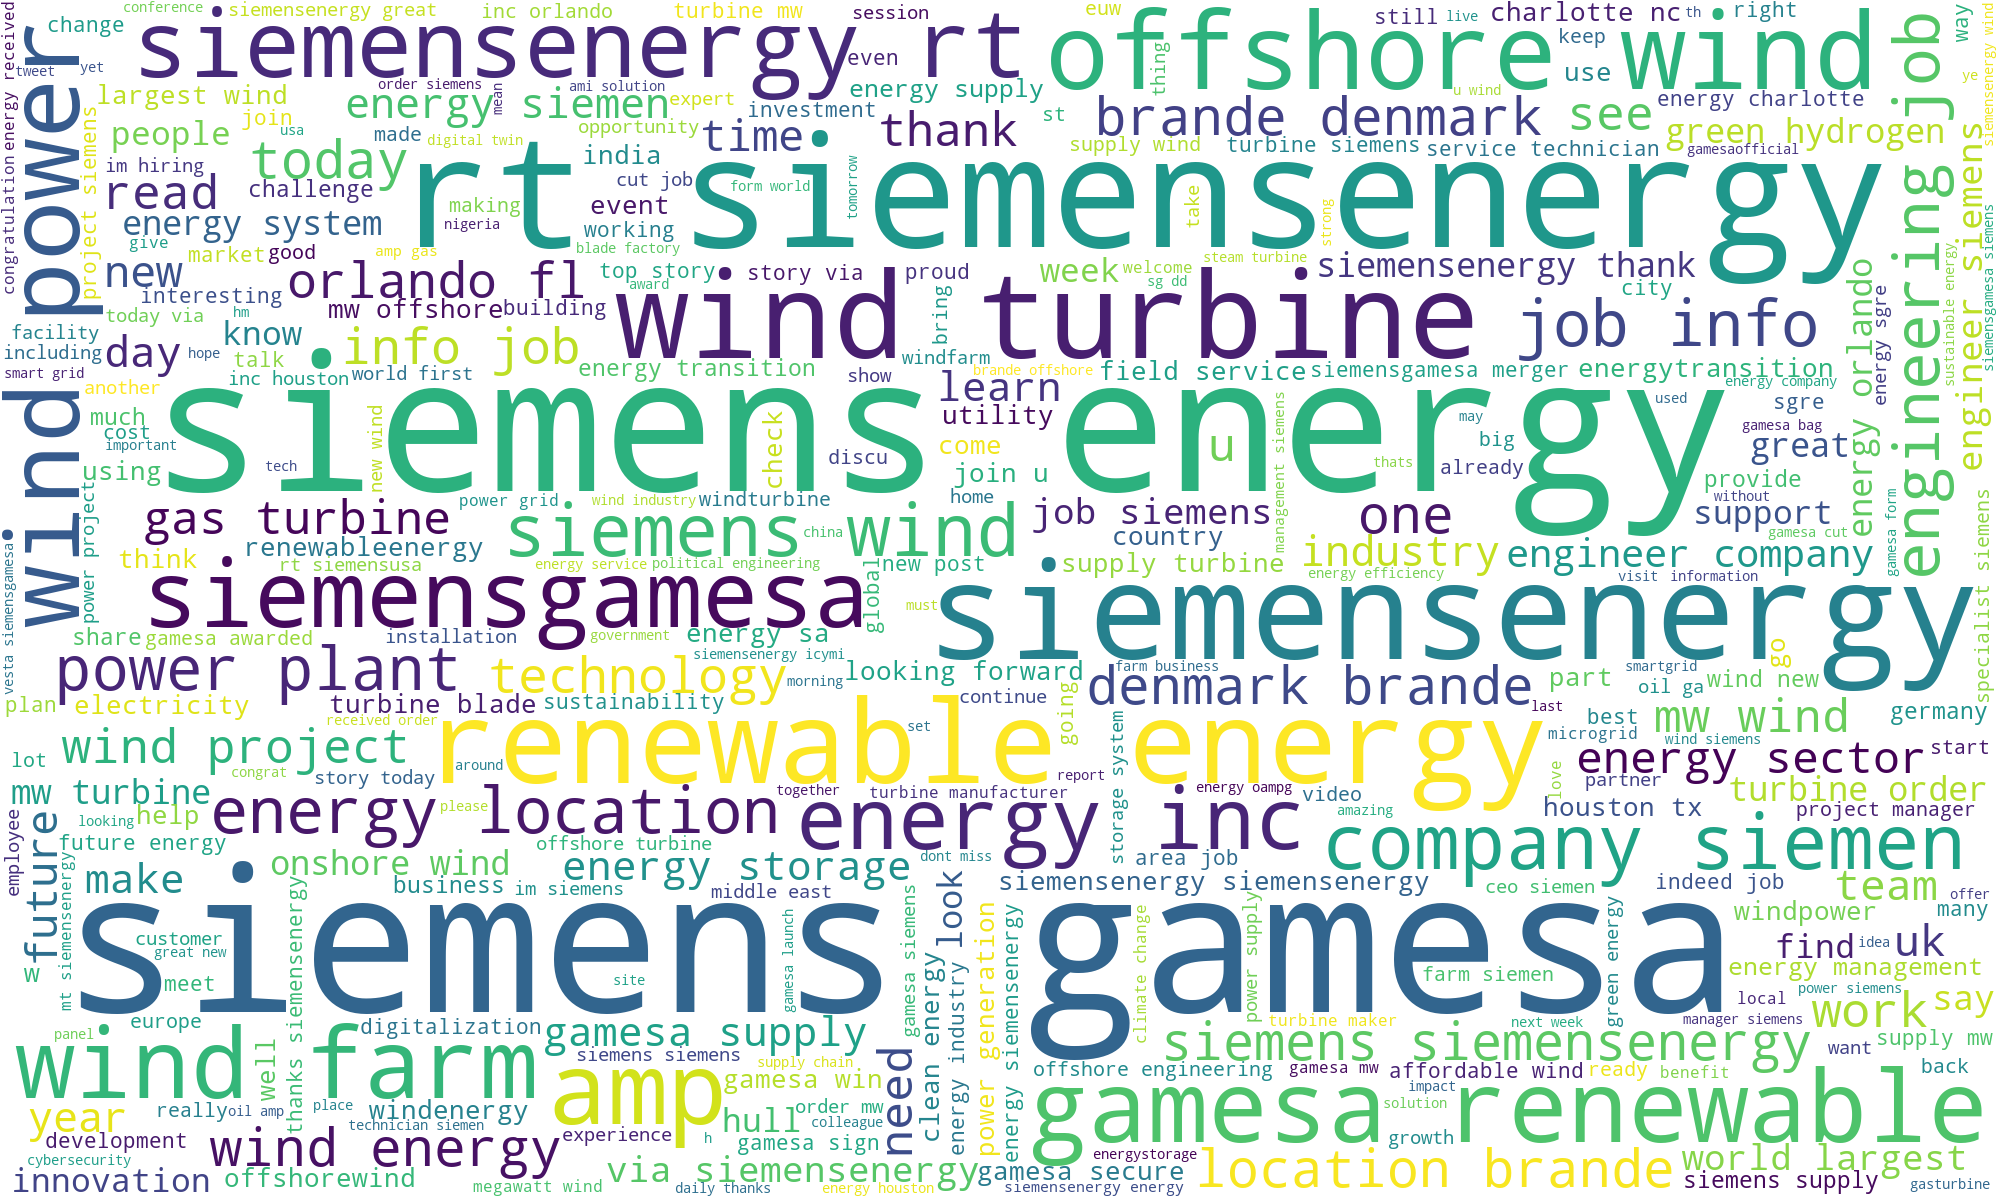
\includegraphics[width=1\linewidth]{images/siemens_gamesa_wordcloud.png}
  \caption{Siemens}
  \label{fig:sfig5}
\end{subfigure}
\begin{subfigure}{0.25\linewidth}
  \centering
  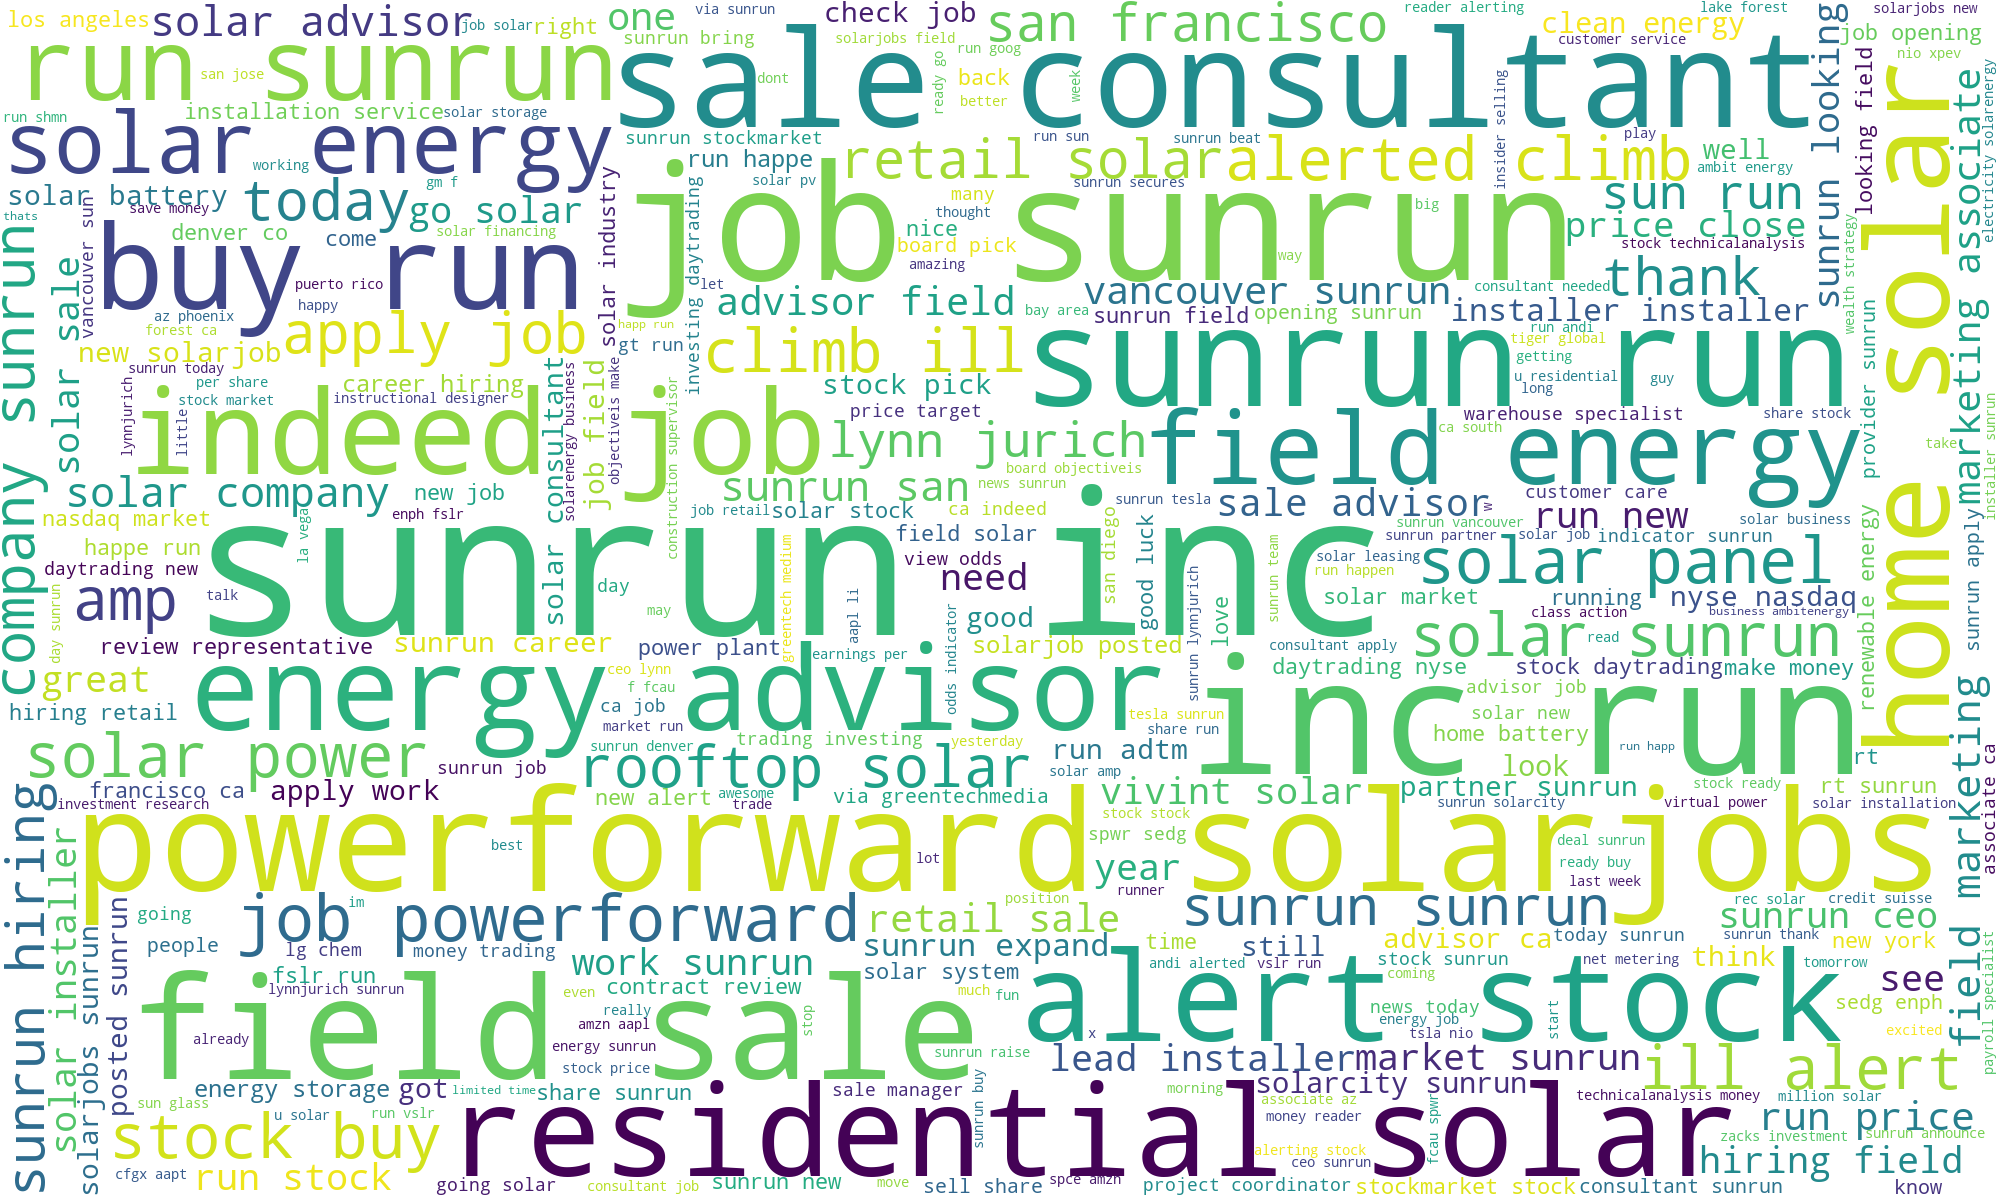
\includegraphics[width=1\linewidth]{images/sunrun_wordcloud.png}
  \caption{Sunrun}
  \label{fig:sfig6}
\end{subfigure}
\caption{Twitter Data - Word Clouds  }
\label{fig:fig}
\end{figure}



\subsubsection{Author id - distribution}
In this small analysis we applied methods for elbow analysis which sets the foundation and is usually used to identify the cut-off for the use of 80-20 rule. The 80-20 rule itself is characterized generally as 80$perc$ of contribution from 20$perc$ population or any data measures for that matter which in our case was for the idea that we were able to find the top 2600 tweet authors that were contributing in forming the 75$perc$ o twitter data that we collected. This analysis cane be useful later when we make modifications to approaches we test for data collected where we can employ these results and collect data only for those 2600 authors or since we know they are sort of the influencers or top contributers that are forming the opinion of the crowd we start following their views directly on other domains and aspects as well. This will turn out to be useful later but fir the scope of this project we have not made use of its discussed applications for now.
\begin{figure}[H]
  \centering
  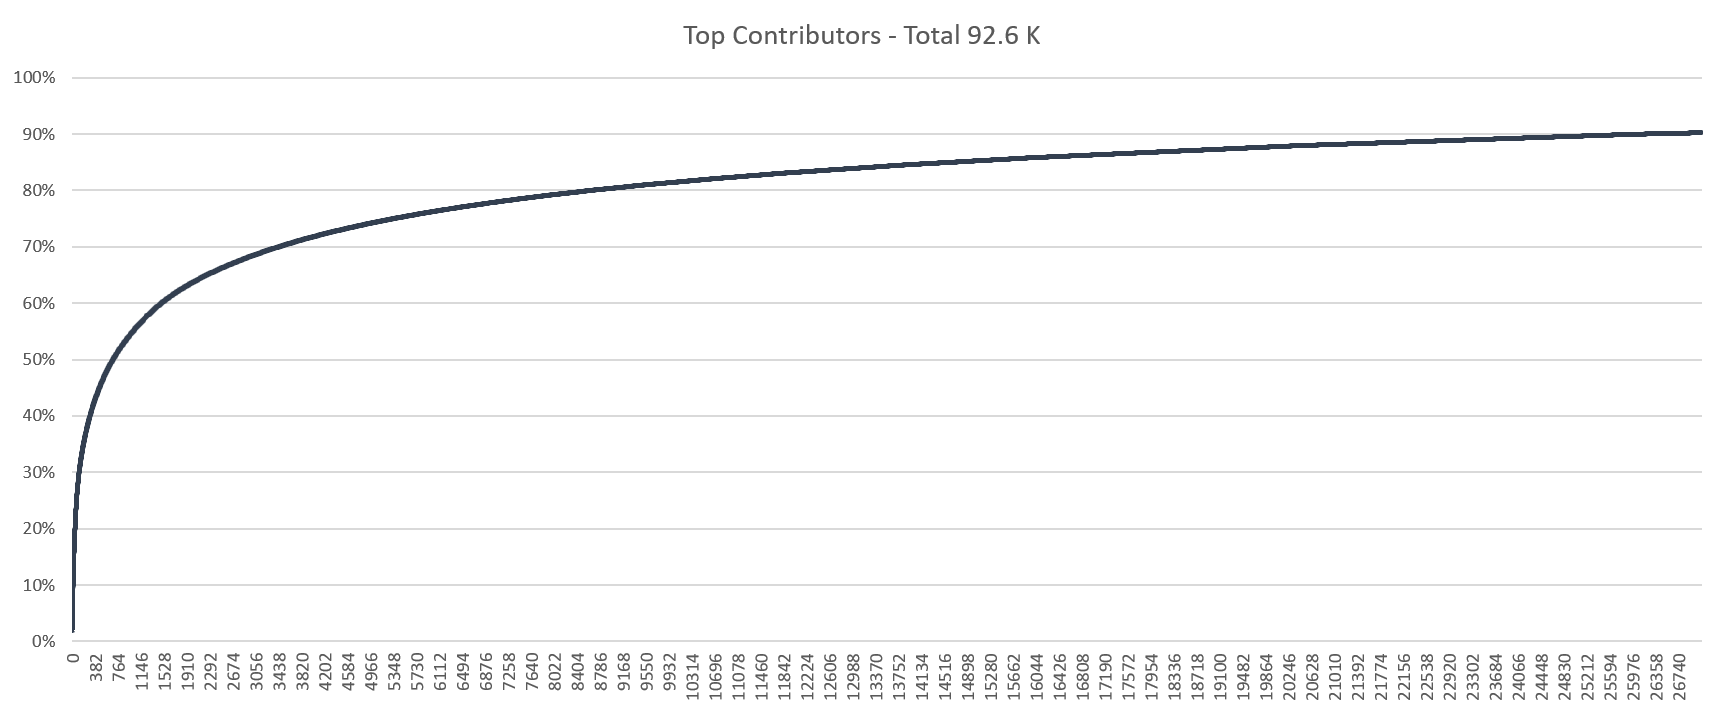
\includegraphics[width=\linewidth]{images/author.png}
  \caption{Tweet Author Importance - 80/20 rule cut-off identification}
%   \label{fig:duck}
\end{figure}



% ========================================================
\section{Data Preparation}
% ========================================================
After having understood the data that we have collected and that which is available to us along with the sense of how we can make it useful for our particular problem we now move on to verify data quality and to remove errors from it so that we are then able to construct the intermediate forms and representations of it which are then finally integrated together to form inputs for the modeling step.
\hl{Must finish}


% --------------------------------------------------------
\subsection{Data selection} % select data
% --------------------------------------------------------
\subsubsection{Twitter Data}
For Twitter data, we retained the following fields:
\begin{enumerate}
    \item Created at
    \item Tweet ID
    \item Author ID
    \item Tweet text
\end{enumerate}

\hl{check for correctness}

\subsubsection{News Article Data}
For news article data, we retained the following fields:

\begin{enumerate}
    \item Date published
    \item Title
    \item Description
\end{enumerate}

\subsubsection{Stock Price Data}
For stock price data, we simply retained all data from the API as they are.

\hl{check for correctness}

% --------------------------------------------------------
\subsection{Clean Data} 
% --------------------------------------------------------
\subsubsection{Twitter and News Article Data}
To perform downstream tasks such as sentiment analysis, the text data from Twitter and news articles must be cleaned. For Twitter, the tweet text was cleaned, and for news articles, the title, combined into one field with the description, was cleaned. We cleaned the data with the following steps:

\begin{enumerate}
    \item Remove punctuation - Remove all punctuations from the sentences.
    \item Tokenization - Transform the sentences into a list of words that can be found in the sentence.
    \item Remove stop words - Remove all English stop words, which do not contribute to the sentiment.
    \item Stemming - Turn all words into their root (stem) form.
    \item Lemmatization - Turn all stem words into dictionary form.
\end{enumerate}



% --------------------------------------------------------
\subsection{Construct Data / Integrate Data } 
% --------------------------------------------------------
%integration's and generalization of scripts
%give what sentiment analysis returned and how it was merged for further analysis
%\\merge all three data sources

\subsubsection{Twitter and News Article Data}
Using the cleaned text data from above, for each entry in the Twitter and news article data we also created a field for sentiment. Using the NLTK SentimentIntensity Analyizer, we found the sentiment for each body of text. These were used to construct time series in modeling.
\hl{double check}

% --------------------------------------------------------
\subsection{Sentiment Analysis} 
% --------------------------------------------------------
The branch of Data Mining corresponding to use of machine learning algorithms to categorize various input samples of relevant text into the dominant and underlying contextual sentiment or notion that characterizes the tone of the text. A sentence “The movie was not bad at all” contains words like bad but the context and underlying notion of it contextually is rather a positive comment regarding it the subject under discussion, hence sentiment analysis makes use of ML techniques, applied strategically and efficiently to classify the text into certain categories of sentiment/nature of the text. Most commonly positive or negative sentiment.
For our project we aimed to experiment and maximize the best approximation by going through various options available in the open-source community but ended up testing two sentiment analyzer tool options available and known as the best ones yet. We chose to employ some of the well established and well known pre-trained sentiment analyzer model available as open-source tools. These included
\begin{enumerate}
    \item Natural Language Tool Kit Sentiment Analyzer for python
    \item Stanford CoreNLP sentiment analyzer
\end{enumerate}

\paragraph{NLTK}
A powerful built-in machine learning operation to obtain insights from linguistic data. It is an open-source library available for python, it is designed to work with human language data making sentiment analysis a necessary tool of it. It provides the complete set of tools required for contextual mining and hence very popular and known for its performance among the text mining community and industry. To be specific we used the \textbf{SentimentIntensityAnalyzer} model instance followed by the polarity score measures it computes.
\\Returned Polarity measures per text sample:
\begin{enumerate}
    \item Positive Sentiment - between 0 and 1 with zero being lowest positivity score and 1 being highest
    \item Negative Sentiment : between 0 and 1 with zero being lowest positivity score and 1 being highest
    \item Compound Sentiment: Less then zero signifies negative sentiment and greater than zero signifies positive sentiment. 0 score value here corresponds to neutral sentiment
    \item Neutral Sentiment
\end{enumerate}
We chose to construct time series for Positive, Negative and Compound sentiments to maximize the potential for finding some useful correlation with any of the three. Neutral Sentiment measure was redundant hence not used further.

\paragraph{Stanford CoreNLP}
CoreNLP enables users to derive linguistic annotations for text, including token and sentence boundaries, parts of speech, named entities, numeric and time values, dependency and constituency parses, co-reference, sentiment, quote attributions, and relations. CoreNLP currently supports 6 languages: Arabic, Chinese, English, French, German, and Spanish. For this analysis we made use of the sentiment annotator of the CoreNLP instance. Although it is a very powerful tool but following are a few issues that came-forth whiles using it which  made us choose and thus opt for the NLTK sentiment analysis and let go of this tool.
\begin{enumerate}
    \item Slow speed
    \item Extensive error debugging required to pin point the issues causing failure of a long run and then restarting the analysis, we did try to do it but it ended being an extensive and extreme wastage of time and resource power of our machines
\end{enumerate}


\subsubsection{Stock Price Data}
Using the "High" and "Low" field in every record, we created a new field "Delta"

$$ Delta = |High - Low|$$

"Delta" returns the absolute value of the change in stock price for a specific stock for that specific day. It can be thought of as a reduction function for the daily high and daily low.

\hl{double check}

% --------------------------------------------------------
\subsection{Format Data } 
% --------------------------------------------------------
Since the stock and Twitter data extend back many years, the granularity of the data was reformatted to be weekly instead of daily. Respective values such as sentiment, delta were averaged over all values for that week.
\hl{double cehck, could maybe delete this section}

% ========================================================
\section{Modeling and Evaluation}
% ========================================================
An integrated model comprising of multiple modeling sub - components has been used to formulate, investigate and analyze the underlying relationship between the stock prices for the top five green industry companies from our list against a few “wisdom of crowd” measures constructed using twitter data; the most significant and useful ones ending up to be the twitter sentiment and entity popularity using tweets. After individually completing the sub-components; the lag analysis and Granger Causality analysis is performed to get a sense of model behavior and its potential to facilitate in making data driven decisions for investment in this industry and particular companies. We make use of the lag analysis with some tweaking and variations, in this section we present in detail some aspects of the approach and techniques we have employed in order to achieve the identified goal.

% --------------------------------------------------------
\subsection{Explore Data Analysis 2 - Explore sentiment data individually} % data exploration report 
% --------------------------------------------------------
To get an idea of the big picture from the sentiment analysis results, we plotted a summary of the positive, negative, and compound Twitter sentiment from 2011 to 2021 in figures \ref{positive_sent_raw} to \ref{comp_sent}, respectively. These plots are specially useful to distinguish an evident anomaly as shown. 

\begin{figure}[H]
  \centering
  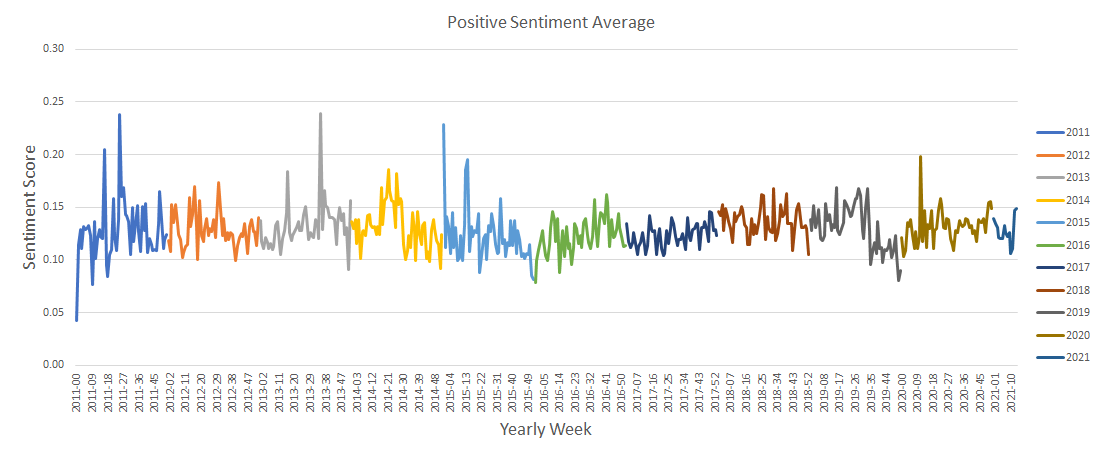
\includegraphics[width=\linewidth]{positive_sent_raw.png}
  \caption{Positive Twitter Sentiment - Year Wise}
  \label{positive_sent_raw}
\end{figure}

\begin{figure}[H]
  \centering
  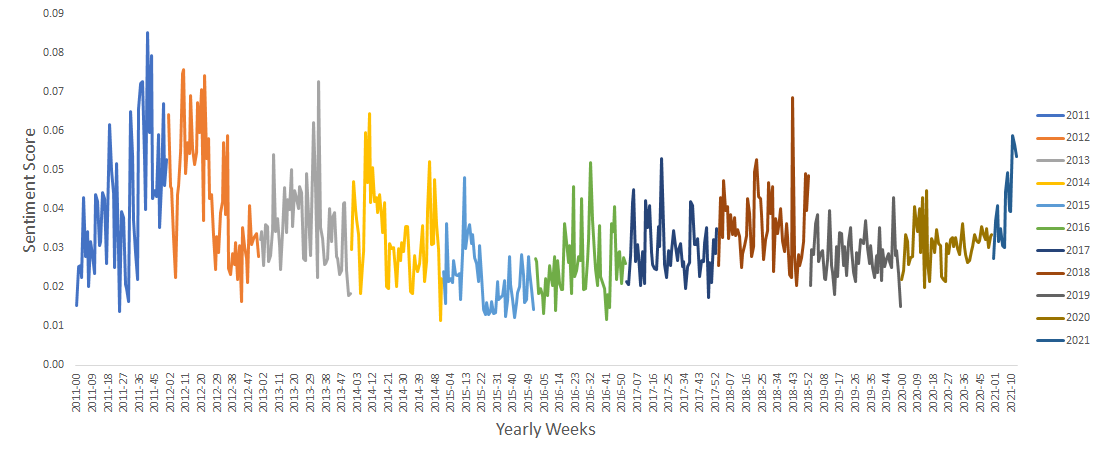
\includegraphics[width=\linewidth]{neg_sent_raw.png}
  \caption{Negative Twitter Sentiment - Year Wise}
  \label{neg_sent_raw}
\end{figure}

\begin{figure}[H]
  \centering
  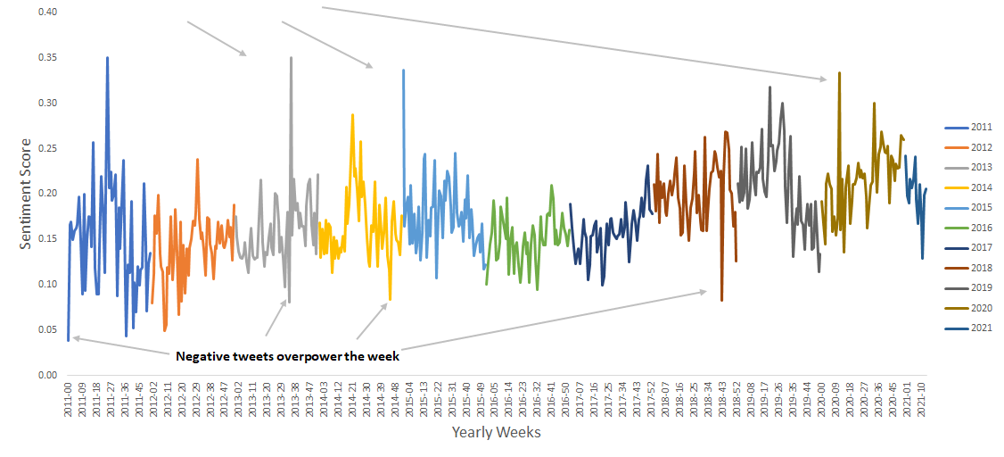
\includegraphics[width=\linewidth]{comp_sent.png}
  \caption{Compound Twitter Sentiment - Year Wise}
  \label{comp_sent}
\end{figure}



% --------------------------------------------------------
\subsection{Twitter Popularity and Stock Prices Series} 
% --------------------------------------------------------
After the initial data exploration. We plotted the Twitter popularity and the stock prices time series. We define the Twitter popularity simply as the daily count of tweets for the respective company. The plots in figures \ref{First Solar Closing Stock Prices_closing_price_daily_tweets} and \ref{Sunpower Closing Stock Prices_closing_price_daily_tweets} show these time series. To the reduce the noise of the daily tweets (popularity), we smooth the series taking the mean of a rolling window of 10 days. \newline 

\textbf{We can observe, as depicted with the red boxes that there is certainly some similarity between the Twitter popularity and the closing stock prices with certain lag. This observation will be investigate using Granger causality, to determine whether the count of daily tweets Granger causes the stock prices.}

\begin{figure}[H]
  \centering
  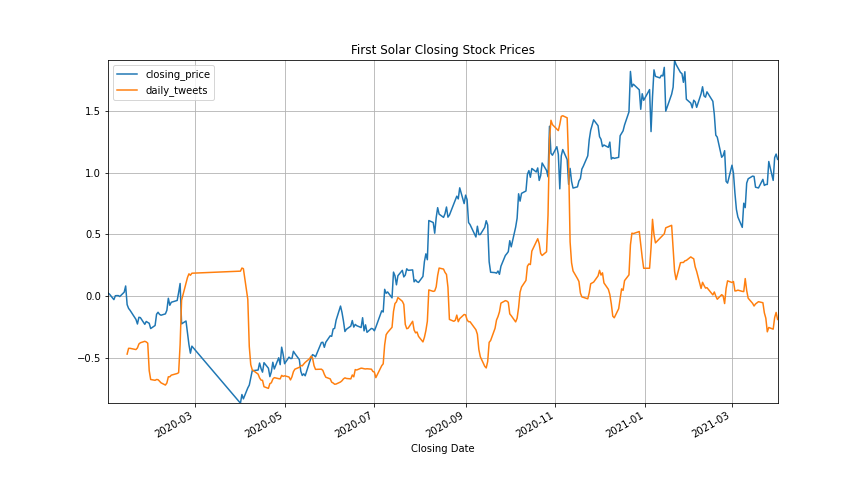
\includegraphics[width=\linewidth, height =1.5in]{popularity_time_series/First Solar Closing Stock Prices_closing_price_daily_tweets.png}
  \caption{First Solar Closing and Popularity Series}
  \label{First Solar Closing Stock Prices_closing_price_daily_tweets} 
\end{figure}

\begin{figure}[H]
  \centering
  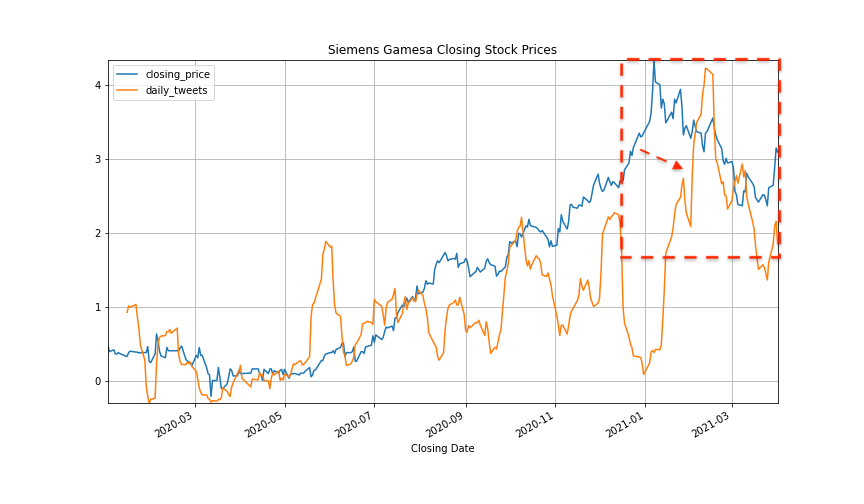
\includegraphics[width=\linewidth, height =1.5in]{popularity_time_series/Siemens Gamesa Closing Stock Prices_closing_price_daily_tweets.png}
  \caption{Siemens Closing and Popularity Series}
  \label{Siemens Gamesa Closing Stock Prices_closing_price_daily_tweets}
\end{figure}

\begin{figure}[H]
  \centering
  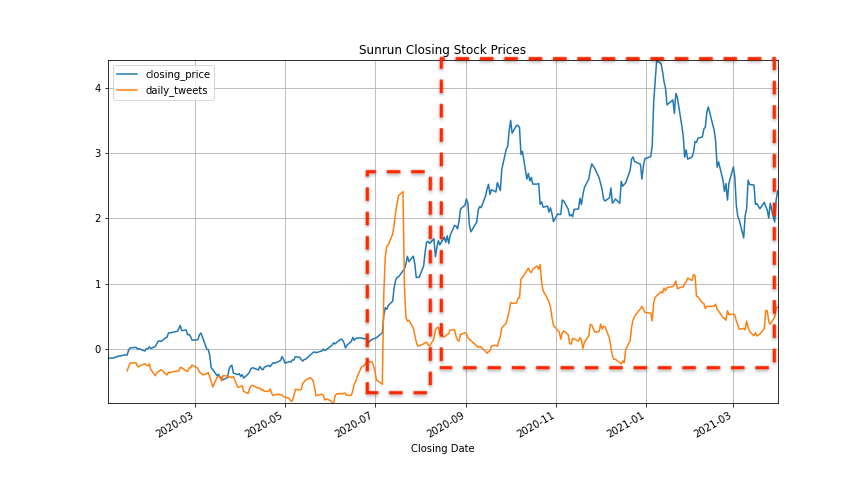
\includegraphics[width=\linewidth, height =1.5in]{popularity_time_series/Sunrun Closing Stock Prices_closing_price_daily_tweets.png}
  \caption{Sunrun Closing and Popularity Series}
  \label{Sunrun Closing Stock Prices_closing_price_daily_tweets}
\end{figure}

\begin{figure}[H]
  \centering
  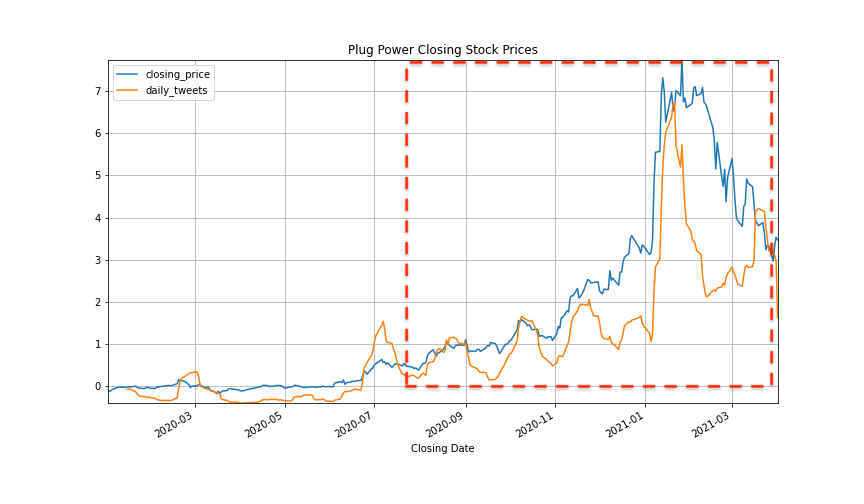
\includegraphics[width=\linewidth, height =1.5in]{popularity_time_series/Plug Power Closing Stock Prices_closing_price_daily_tweets.png}
  \caption{Plug Power Closing and Popularity Series}
  \label{Plug Power Closing Stock Prices_closing_price_daily_tweets}
\end{figure}

\begin{figure}[H]
  \centering
  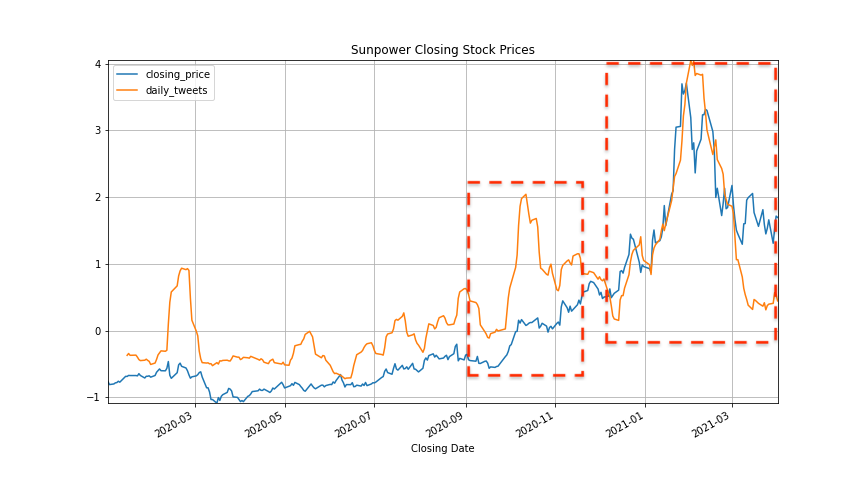
\includegraphics[width=\linewidth, height =1.5in]{popularity_time_series/Sunpower Closing Stock Prices_closing_price_daily_tweets.png}
  \caption{Sunpower Closing and Popularity Series}
  \label{Sunpower Closing Stock Prices_closing_price_daily_tweets}
\end{figure}


% --------------------------------------------------------
\subsection{Compound Sentiment and Stock Prices Series} 
% --------------------------------------------------------
We followed a similar approach to that of the previous section the compound sentiment and closing stock prices. Nevertheless,  just by inspection, there is not many clear similarities in the two series. This observation will be investigated as well in the next sections.

\begin{figure}[H]
  \centering
  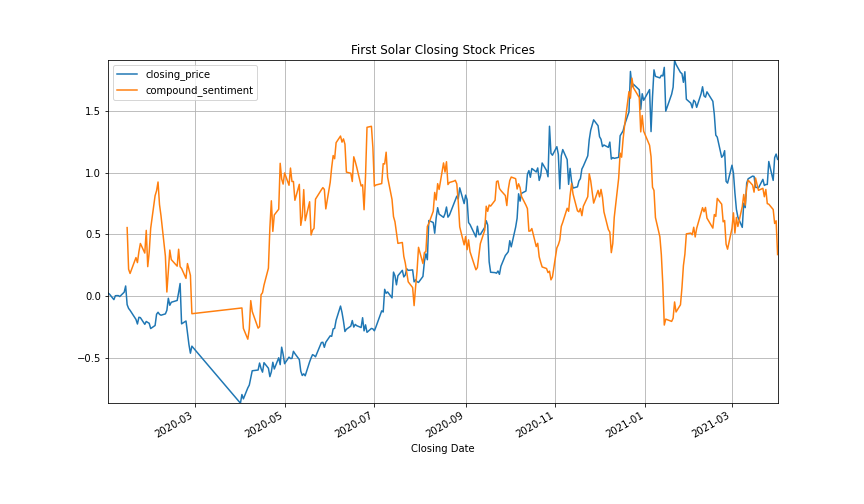
\includegraphics[width=\linewidth, height =1.5in]{sentiment_time_series/First Solar Closing Stock Prices_closing_price_compound_sentiment.png}
  \caption{First Solar Closing and Sentiment Series}
\end{figure}

\begin{figure}[H]
  \centering
  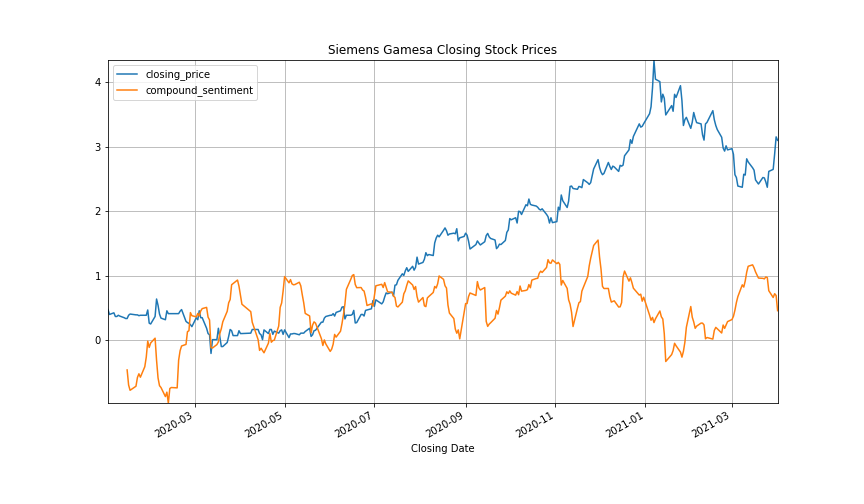
\includegraphics[width=\linewidth, height =1.5in]{sentiment_time_series/Siemens Gamesa Closing Stock Prices_closing_price_compound_sentiment.png}
  \caption{Siemens Closing and Sentiment Series}
\end{figure}

\begin{figure}[H]
  \centering
  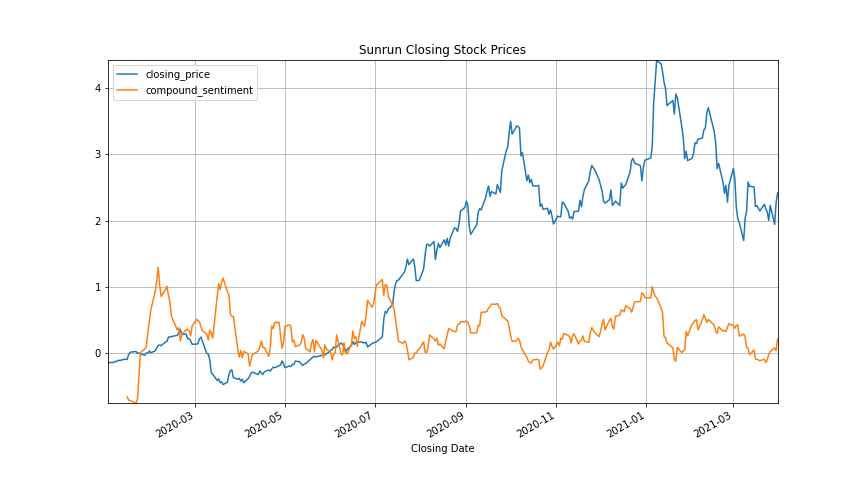
\includegraphics[width=\linewidth, height =1.5in]{sentiment_time_series/Sunrun Closing Stock Prices_closing_price_compound_sentiment.png}
  \caption{Sunrun Closing and Sentiment Series}
\end{figure}

\begin{figure}[H]
  \centering
  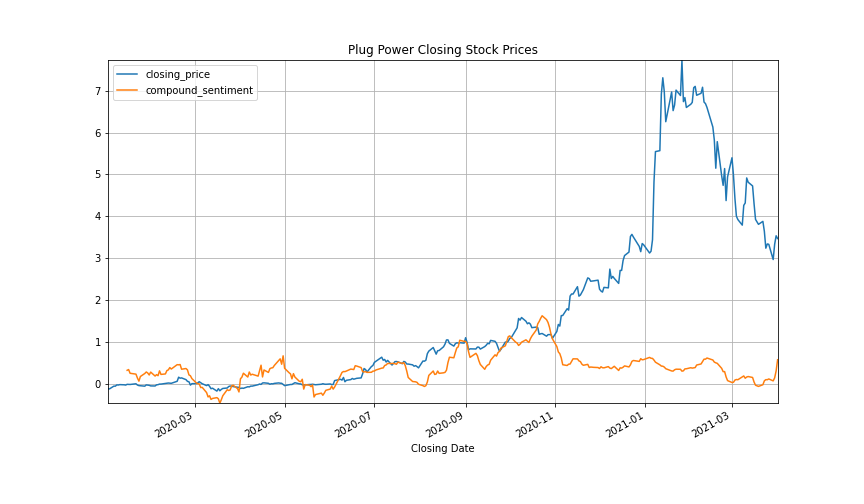
\includegraphics[width=\linewidth, height =1.5in]{sentiment_time_series/Plug Power Closing Stock Prices_closing_price_compound_sentiment.png}
  \caption{Plug Power Closing and Sentiment Series}
\end{figure}

\begin{figure}[H]
  \centering
  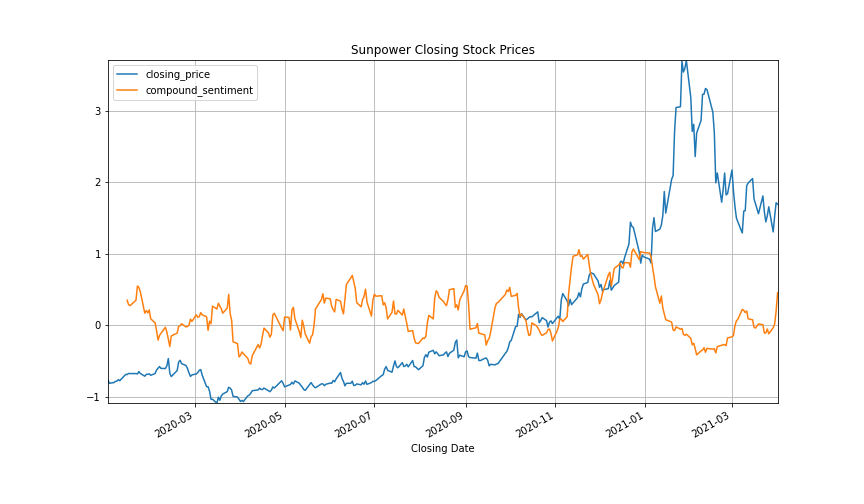
\includegraphics[width=\linewidth, height =1.5in]{sentiment_time_series/Sunpower Closing Stock Prices_closing_price_compound_sentiment.png}
  \caption{Sunpower Closing and Sentiment Series}
  \label{Sunpower Closing Stock Prices_closing_price_compound_sentiment}
\end{figure}

% --------------------------------------------------------
\subsection{Lag and Correlation Analysis} 
% --------------------------------------------------------
A distributed lag model is a model for time series data in which a regression equation is used to predict current values of a dependent variable based on both the current values of an explanatory variable and the lagged (past period) values of this explanatory variable.

\textbf{"After extensive lag analysis and simplifying the convoluted and counter intuitive results that we were getting, we were able to conclude that the green energy industry as a whole has just picked up the pace. This has been observed in the data, as illustrated in figures \ref{all_stock_prices_2015_2021} to \ref{all_stock_prices_2020_2021},  and is transforming the usefulness of our approach from long term uniformity that we witnessed of stock prices for these companies in the open market into a much shorter term predictive capability; very slightly now (given the recent awareness and shift, July 2020 on-wards) but very surely so. Given a few more years for this industry to mature, this same approach we have presented in the paper will be capable of short term predictive usefulness for driving short term insightful decisions as well. "}


\begin{figure}[H]
  \centering
  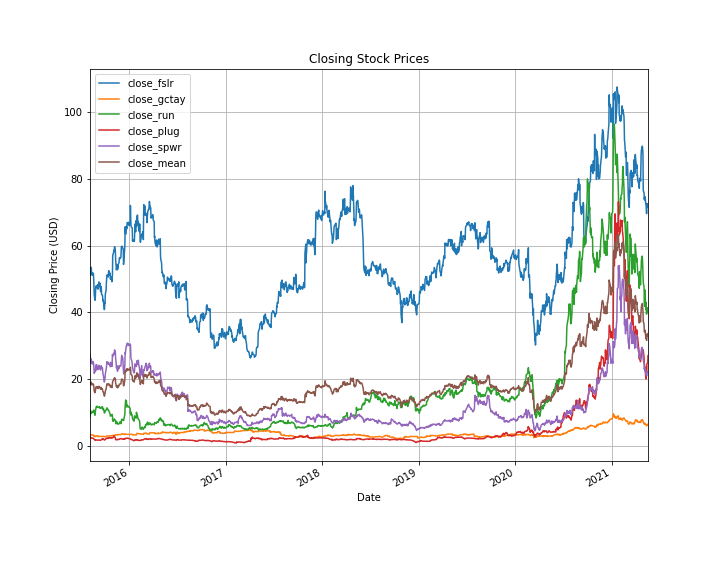
\includegraphics[width=\linewidth]{all_stock_prices_and_mean/all_stock_prices_2015_2021.png}
  \caption{All Stock Prices - 2015 to 2021}
  \label{all_stock_prices_2015_2021}
\end{figure}

\begin{figure}[H]
  \centering
  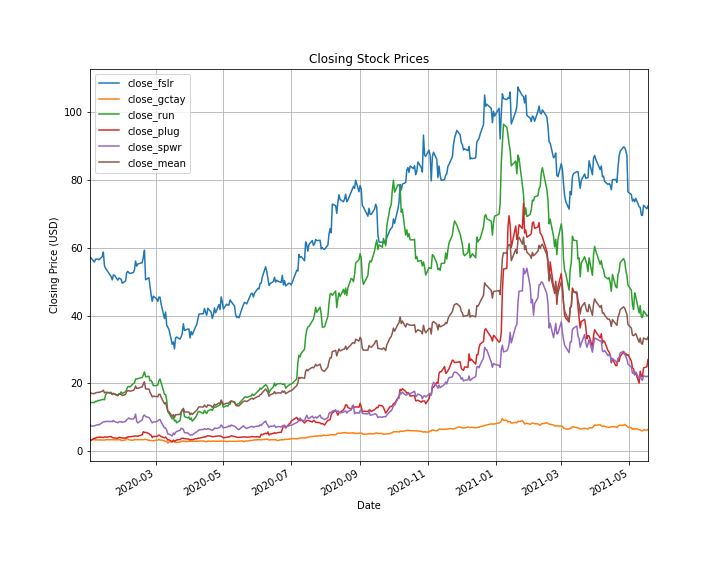
\includegraphics[width=\linewidth]{all_stock_prices_and_mean/all_stock_prices_2020_2021.png}
  \caption{Significant Pace of Volatility in all green energy companies in later half of 2020}
  \label{all_stock_prices_2020_2021}
\end{figure}

\subsubsection{Popularity Vs. Closing Price}
\subsubsection{Sentiment Vs. Closing Price}
In this section, we present the various combinations we tested for the lag analysis of each company against the positive, negative and compound sentiments (figures \ref{fslr_100_pos} to \ref{srun_1000_comp}) respectively and discuss what insights it provides us for figuring out the underlying correlation. For every company,  we plotted a lag analysis initially for a max lag of 100 against stock-prices and each sentiment(Positive, Negative and Compound) but realized that the distribution of correlation is somewhat constant over this time and it only slightly varies towards the positive lag values. \newline

It was difficult to comprehend why this was but then plotting lag analysis with max-lag values of greater time periods like 500 days and 1000 days we saw a better distribution that made sense. This allowed us to understand that the current relationship between stock prices and sentiments is stable and slow-changing. The market gap is easily 100 days which sounds pretty off but when analyzed against the raw stock prices we had for the companies and their insignificance and awareness in the market people and investors validated the fact that the very last months of 2020 i.e to be specific from July 2020 on-wards we see a significance movement in the majority companies' stock prices which reinforces and validates the consistent distribution of correlation in lag analysis. \newline

That consistent part highlights the idea that people started talking about these green companies earlier and have been for a while but it never translated into action of investment that might be significant in contribution and growth of the stock itself, the true investment action although volatile in nature such that it is following cycles of rise and fall in the time period after July 2020 to latest days although does prove to now give us some useful material for varying correlation. \newline

The uniformity of the stock prices in the majority of the time overpowered and not much useful and significant relationship in the short term cut-offs rather long term correlation is pretty much meaningful and so what we concluded overall from all the analysis that will now be listed and below we concluded that the green-investing energy is not quite volatile at the moment and the decision making can be done for the longer term rather short term given the current talk in the town and awareness in the audience we have taken under consideration. \newline 

Simply put we have identified that there has been some shift in the attitude of the investors towards this green industry from July 2020 on-wards although volatile in this shorter time period but still now people are talking about it. Whereas for the majority preceding chunk of time there was uniformity in the green industry not making analysis like ours useful but this shift that we have been able to recognize in the attitude of people towards this industry and its reinforcements from the data validates that giving some more time to this industry i.e a few years or so it will be very useful to have an analysis replicated as ours which would then start indication short-term correlation and decision making. \newline

So finally setting it straight the current analysis leans towards helping us gain long-term insights on the stocks and if we give some time to this green industry we can reuse this same approach and we will most likely be able to present short-term insights gained with a reduced market gap. Right now our market gap is in unit of years basically rather than days but once the industry grows further given the trend we started observing from later half of 2020 it should easily reduce down to weeks and days etc. Any day we choose as optimal lag value for now between 0 - 100 or so will be giving us the same insights so the daily volatility becomes insignificant and hence we can get a longer term picture for now because what correlation we might get for a day 200 days away from the chosen one is where we start seeing decline rather than the very next day. Our lag analysis basically done on yearly or half year granularity would have given us something we expect as the change with smaller number of point until max lag. So imagine we have the lag analysis chart below and every line pair of consecutive lines/points are time wise at a distance of 6 months.
\newline

\subsubsection{Discussion for Lag and Correlation analysis } 
All except First Solar in figure \ref{all_stock_prices_2015_2021} recently gained the pace and that was an interesting find which made sense to the uniformity of the lag analysis over shorter chunks of time. Where a lag of one or hundred would end up giving the same results as compared to obvious delta and declining correlation in increasing lags significantly to greater lag ranges.
Figure \ref{all_stock_prices_2015_2021} illustrates that something is going on the crowds very recently that is reflected in people now buying and selling more of the green energy company stocks as opposed to the non-popularity and uniformity they were facing in the previous years. This phenomenon is visible in figure \ref{all_stock_prices_2015_2021} and \ref{all_stock_prices_2020_2021} very clearly. The lag analysis' slight variations on one half of the plot in the 100 lag category reinforces this as well. The position of this half decreasing curve formed in the following lag analysis will vary depending on whether we are plotting the price against positive or negative sentiment. As ample for two of the companies is attached below with the rest available in appendix. \newline

% \begin{figure}[H]
%   \centering
%   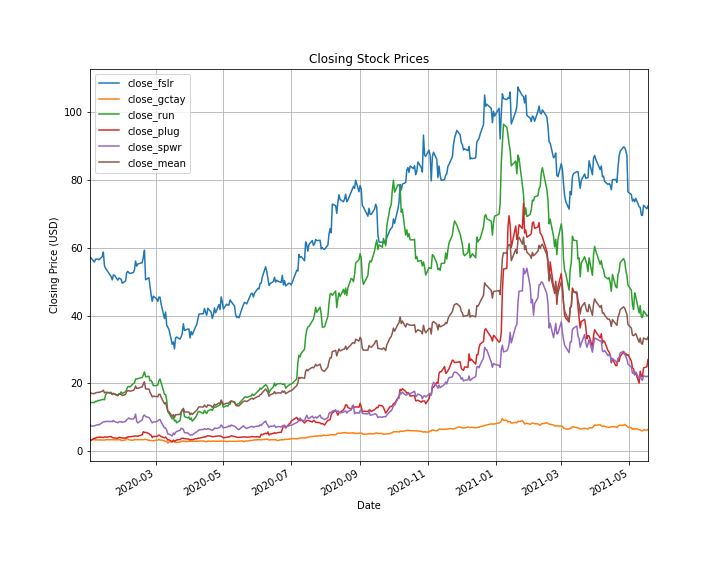
\includegraphics[width=\linewidth]{all_stock_prices_and_mean/all_stock_prices_2020_2021.png}
%   \caption{Significant Pace of Volatility in all green energy companies in later half of 2020}
% %   \label{fig:duck}
% \end{figure}

\newline
\textbf{Lag Analysis For First Solar}
%--------------- FSLR Positive _-------------------
\begin{figure}[H]
  \centering
  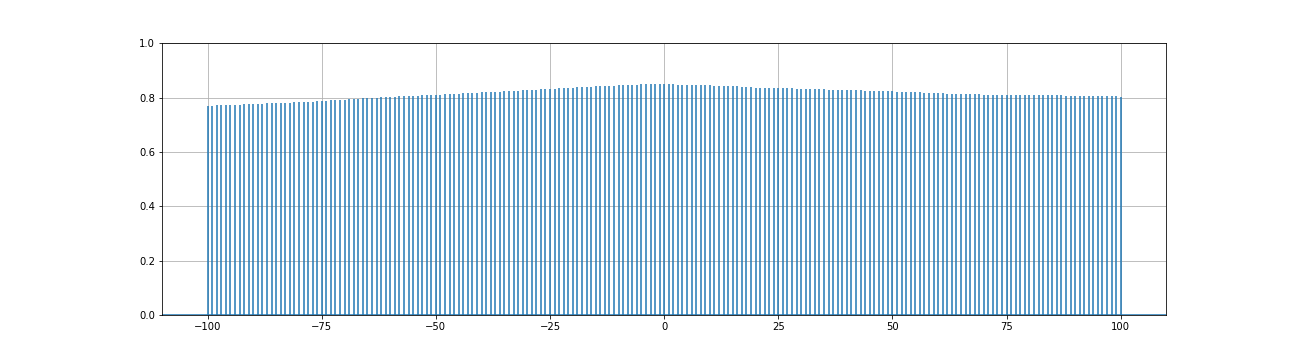
\includegraphics[width=\linewidth]{images/fslr_100_pos.png}
  \caption{First Solar - Positive Vs Closing Price - Max Lag =100}
  \label{fslr_100_pos}
\end{figure}

\begin{figure}[H]
  \centering
  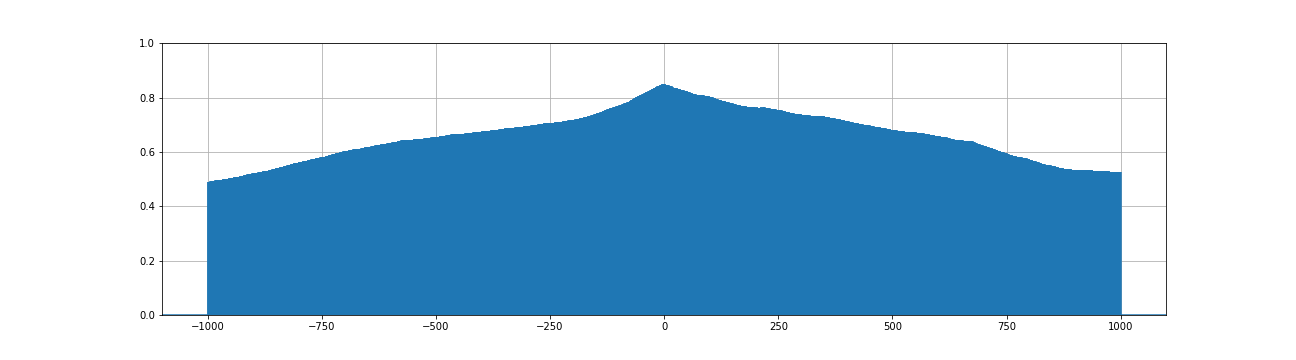
\includegraphics[width=\linewidth]{images/fslr_1000_pos.png}
  \caption{First Solar - Positive Vs Closing Price - Max Lag =1000}
  \label{fslr_1000_pos}
\end{figure}

%--------------- FSLR Positive  End -------------------


%--------------- FSLR Negative -------------------

\begin{figure}[H]
  \centering
  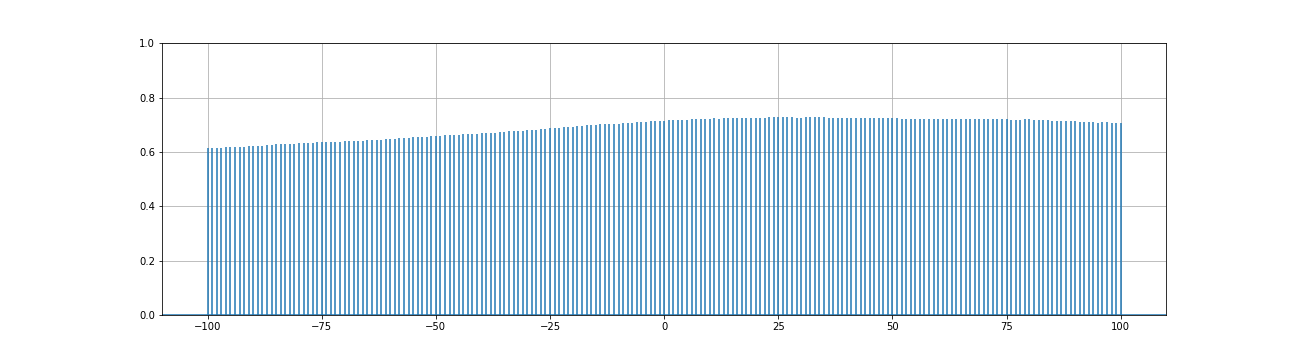
\includegraphics[width=\linewidth]{images/fslr_100_neg.png}
  \caption{First Solar - Negative Vs CLosing Price - Max Lag =100}
  \label{fslr_100_neg}
\end{figure}

\begin{figure}[H]
  \centering
  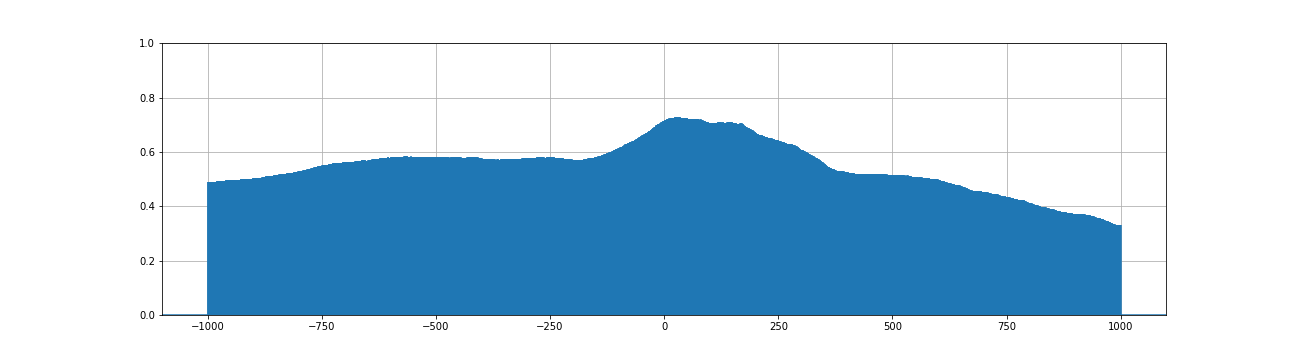
\includegraphics[width=\linewidth]{images/fslr_1000_neg.png}
  \caption{First Solar - Negative Vs Closing Price - Max Lag =1000}
  \label{fslr_1000_neg}
\end{figure}
%--------------- FSLR Negative End  -------------------

'%--------------- FSLR Compound -------------------
\begin{figure}[H]
  \centering
  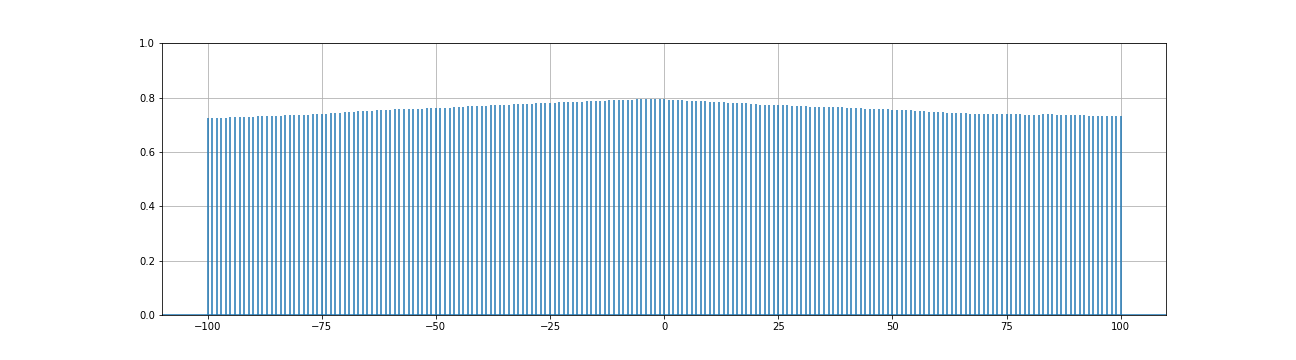
\includegraphics[width=\linewidth]{images/fslr_100_comp.png}
  \caption{First Solar - Compound Vs CLosing Price - Max Lag =100}
  \label{fslr_100_comp}
\end{figure}

\begin{figure}[H]
  \centering
  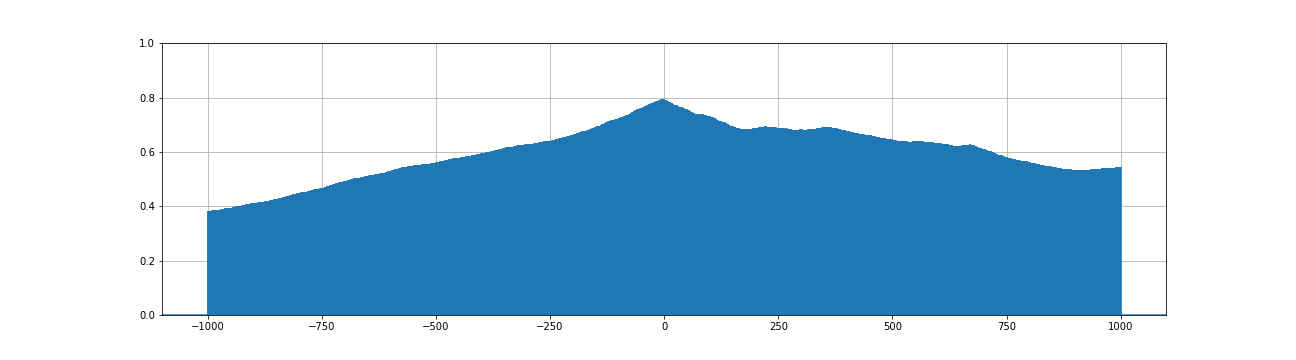
\includegraphics[width=\linewidth]{images/fslr_1000_comp.png}
  \caption{First Solar - Compound Vs Closing Price - Max Lag =1000}
  \label{fslr_1000_comp}
\end{figure}
%--------------- FSLR Compound  End -------------------





\textbf{Lag Analysis For Sun Run}
\newline
%--------------- SunRun Positive _-------------------
\begin{figure}[H]
  \centering
  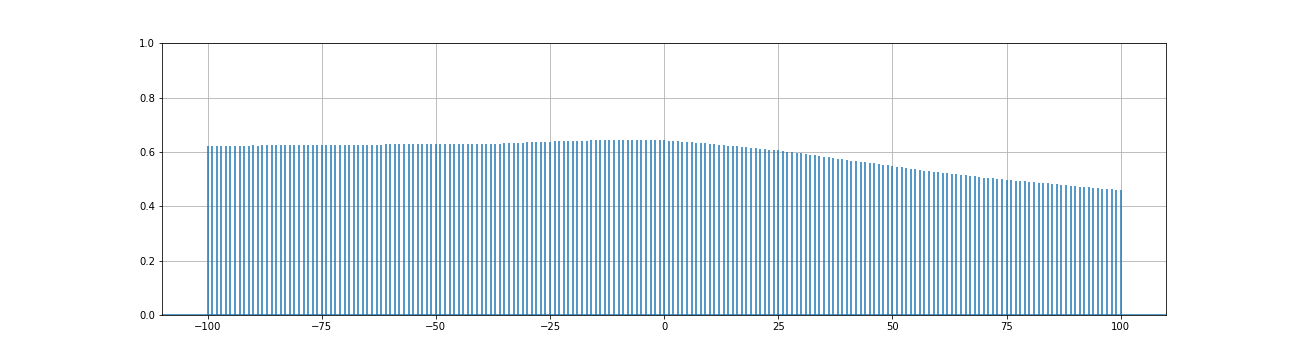
\includegraphics[width=\linewidth]{images/srun_100_pos.png}
  \caption{Sun Run - Positive Vs Closing Price - Max Lag =100}
  \label{srun_100_pos}
\end{figure}

\begin{figure}[H]
  \centering
  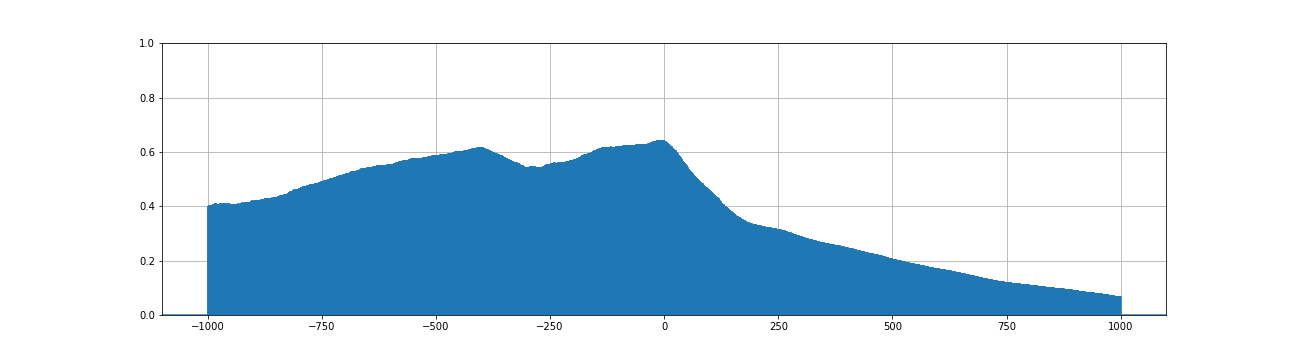
\includegraphics[width=\linewidth]{images/srun_1000_pos.png}
  \caption{Sun Run - Positive Vs Closing Price - Max Lag =1000}
  \label{srun_1000_pos}
\end{figure}

%--------------- SunRun Positive  End -------------------


%--------------- SunRun Negative Begin -------------------

\begin{figure}[H]
  \centering
  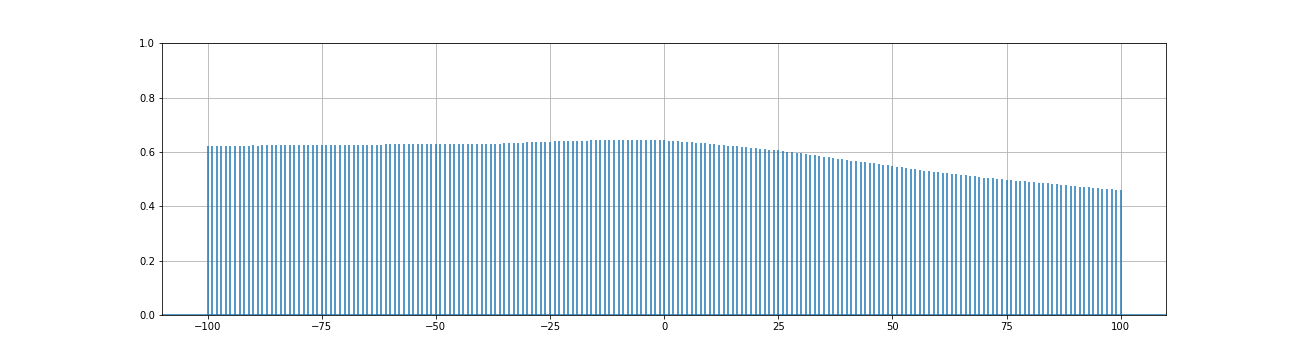
\includegraphics[width=\linewidth]{images/srun_100_pos.png}
  \caption{Sun Run - Negative Vs CLosing Price - Max Lag =100}
  \label{srun_100_pos}
\end{figure}

\begin{figure}[H]
  \centering
  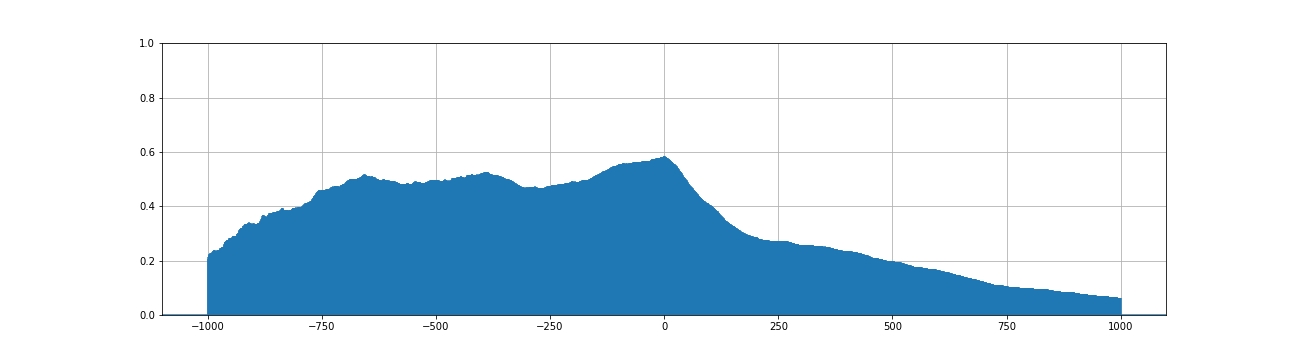
\includegraphics[width=\linewidth]{images/srun_1000_neg.png}
  \caption{Sun Run - Negative Vs Closing Price - Max Lag =1000}
  \label{srun_1000_neg}
\end{figure}
%--------------- SunRun Negative End  -------------------

'%--------------- SunRun Compound -------------------
\begin{figure}[H]
  \centering
  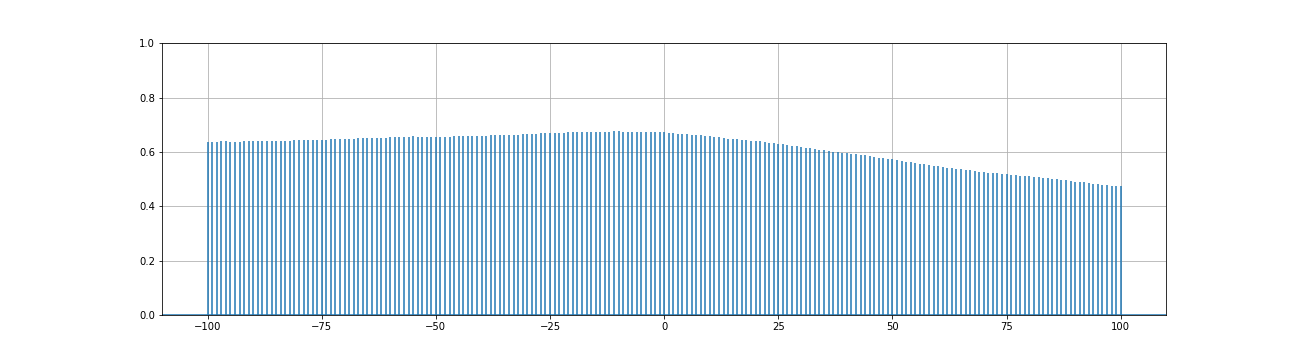
\includegraphics[width=\linewidth]{images/srun_100_comp.png}
  \caption{Sun Run - Compound Vs CLosing Price - Max Lag =100}
  \label{srun_100_comp}
\end{figure}

\begin{figure}[H]
  \centering
  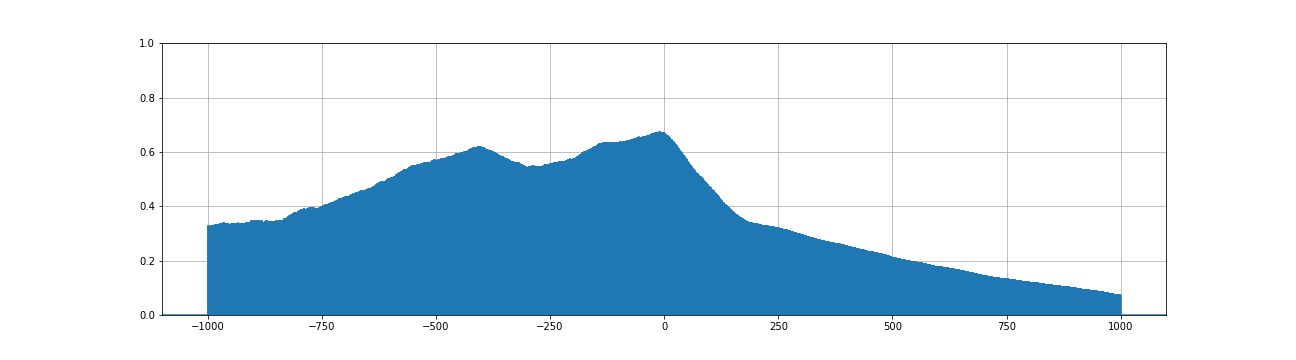
\includegraphics[width=\linewidth]{images/srun_1000_comp.png}
  \caption{Sun Run - Compound Vs Closing Price - Max Lag =1000}
  \label{srun_1000_comp}
\end{figure}
%---------------SunRun Compound  End -------------------




% --------------------------------------------------------
\subsection{Granger Causality} 
% --------------------------------------------------------
The Granger causality results are presented in figures \ref{granger_first_solar} to \ref{granger_sunpower}. For each of the companies we did four F-tests. We used compound, positive, negative sentiment, as well as daily tweets to determine whether each series Granger causes the closing prices. The determine whether one of these series Granger causes closing prices, we looked for lag values which have a very low p value $(p < 0.05)$. Those lag with their respective $p$ and $F$ values are shown in the figures  \ref{granger_first_solar} to \ref{granger_sunpower}. \newline

For each company, different series Granger causes the closing prices at different lags so we cannot make a definitive claim about the effectiveness of one series with respect to another one for all of the companies. Nevertheless, we can observe that the amount of daily tweets is the most successful at Granger causing the closing prices except for First Solar.  It is worth noting that the figure only some of the lags with $p < 0.05$. \newline

\textbf{We can indeed check that the lag values output by the F-test do make sense with the time series plot in figures \ref{First Solar Closing Stock Prices_closing_price_daily_tweets} to \ref{Sunpower Closing Stock Prices_closing_price_compound_sentiment}. Specifically, we can observe that the lag values do match with the shift of the daily tweets and the closing prices, indicating that twitter popularity does predict up to a certain extent the closing prices. In general, we can also see that sentiment score shows to be less effective at Granger causing values of closing prices, and that for the companies Sunrun, Plug Power, and Sunpower, the sentiment scores is not relevant at all for this scenario.}

\begin{figure}[H]
  \centering
  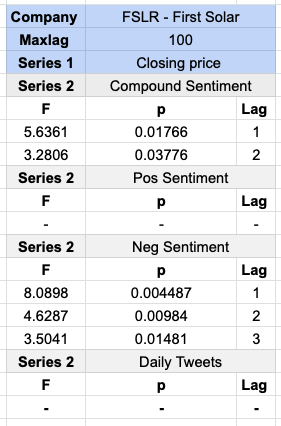
\includegraphics[width=0.4\linewidth]{granger_results/granger_first_solar.png}
  \caption{Granger Results - First Solar}
  \label{granger_first_solar}
\end{figure}

\begin{figure}[H]
  \centering
  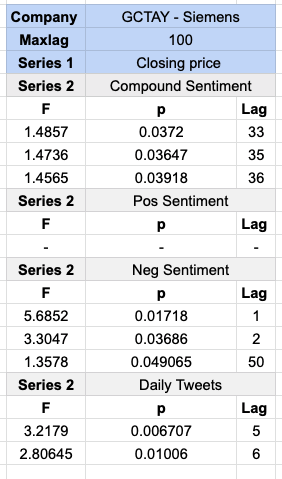
\includegraphics[width=0.4\linewidth]{granger_results/granger_siemens.png}
  \caption{Granger Results - Siemens}
  \label{granger_siemens}
\end{figure}

\begin{figure}[H]
  \centering
  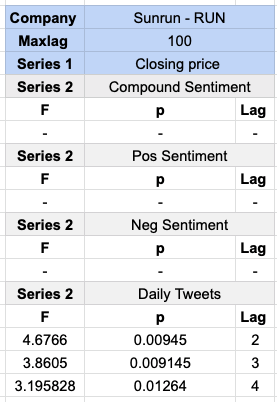
\includegraphics[width=0.4\linewidth]{granger_results/granger_sunrun.png}
  \caption{Granger Results - Sunrun}
  \label{granger_sunrun}
\end{figure}

\begin{figure}[H]
  \centering
  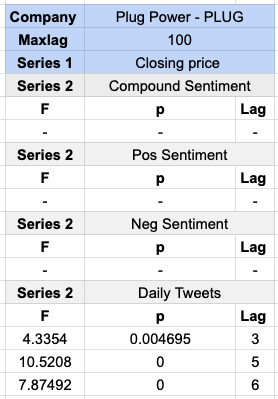
\includegraphics[width=0.4\linewidth]{granger_results/granger_plug.png}
  \caption{Granger Results - Plug Power}
  \label{granger_plug}
\end{figure}

\begin{figure}[H]
  \centering
  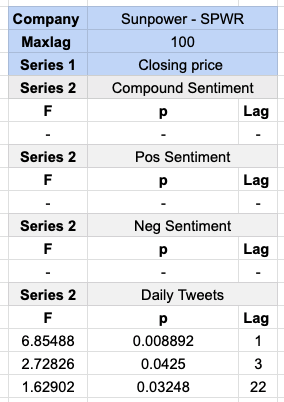
\includegraphics[width=0.4\linewidth]{granger_results/granger_sunpower.png}
  \caption{Granger Results - Sunpower}
  \label{granger_sunpower}
\end{figure}


\subsubsection{Discussion for Granger Causality analysis:}

% --------------------------------------------------------
\subsection{TF-IDF: Term frequency–inverse document frequency} 
% --------------------------------------------------------
We also performed $TF\_IDF$ to get key word extraction, the results are as below and this can be further used to develop more insightful analysis but for this project due to limited time we plan on making use of it creatively for extension of the project to new aspects.

\newline 
Top 20 key words for each company have been computed but it varies depending on the importance returned, they might be and usually were less than 20.
\begin{figure}[H]
  \centering
  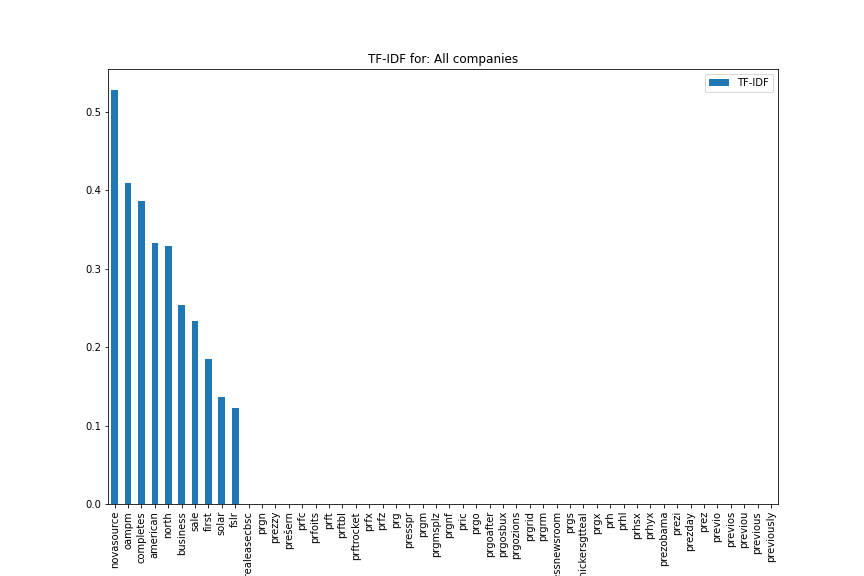
\includegraphics[width=\linewidth, height =1.5in ]{all_tfidf.png}
  \caption{TF-IDF - All companies}
%   \label{fig:duck}
\end{figure}
\begin{figure}[H]
  \centering
  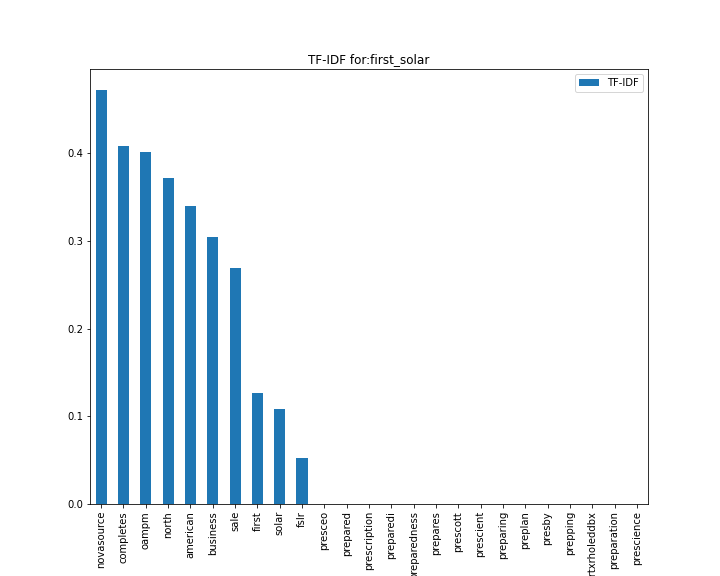
\includegraphics[width=\linewidth, , height =1.5in]{first_solartfidf.png}
  \caption{TF-IDF - First Solar}
%   \label{fig:duck}
\end{figure}
\begin{figure}[H]
  \centering
  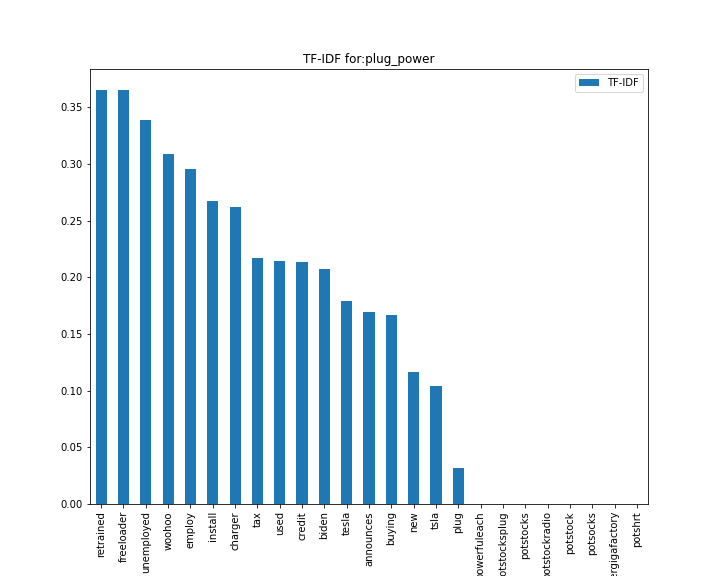
\includegraphics[width=\linewidth, height =1.5in]{plug_powertfidf.png}
  \caption{TF-IDF - Plug Power}
%   \label{fig:duck}
\end{figure}
\begin{figure}[H]
  \centering
  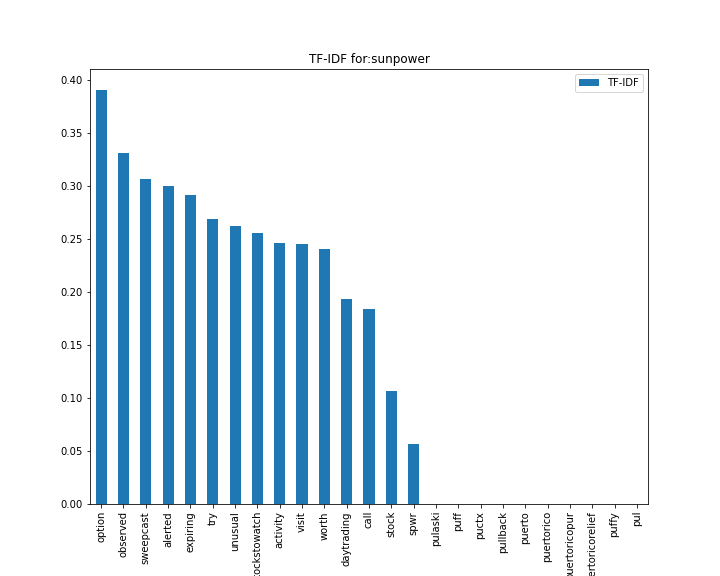
\includegraphics[width=\linewidth, height =1.5in]{sunpowertfidf.png}
  \caption{TF-IDF - Sun Power}
%   \label{fig:duck}
\end{figure}
\begin{figure}[H]
  \centering
  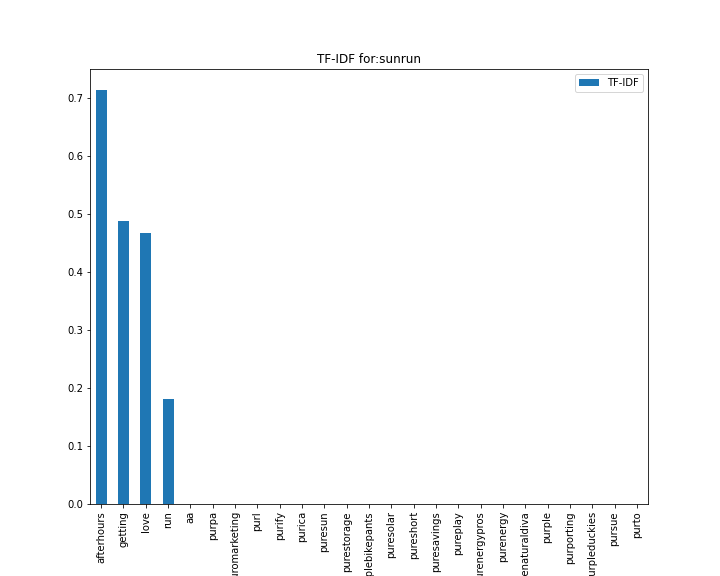
\includegraphics[width=\linewidth, height =1.5in]{sunruntfidf.png}
  \caption{TF-IDF - Sun Run}
%   \label{fig:duck}
\end{figure}




% ========================================================
\section{Conclusion}
% ========================================================
After doing extensive work on implementing the methodology we had in mind for solving the identified problem statement of \textbf{"Using Twitter and news article data to predict stock market prices for green energy companies”} we have understood the underlying relationship to some extent after several iterations. The main highlights were that we see good results conforming to all the series of analysis we applied in the way to reach the final comparative time series plots. An interesting learning point was that due to pre2020-July period for the green energy industry there was not much going on and so very little margin to explore the highest potential of data driven decisions but the post July-2020 times did put a lot in perspective and so we also see that towards the ;after end of the Time series there is significant similarity between the closing stock prices and the popularity and sentiment measures. There was similarity and this similarity in trend had to be validated using to know whether the metrics that we are testing are the ones actually causing the change as well or not, this was done using Granger Causality and we were hence able to conclude from the results of Granger Causality analysis that our metrics are indeed the Granger Cause for the rise and fall which gives us immense power to manipulate this predictive insight and use it refined data driven decision that are better than intuition of investors and if not even better, they complement their intuition as well. Another learning point it highlight is that the causation pattern indeed is not exactly similarly driven for every company in regard to stock prices, for some its extremely aligned like Plug Power and Sun Power( Fig 31 a and b) whereas for others its matching the pace to some extent. Hence, we would say that this series of analysis proves to be quite useful and can be further refined and tuned to perform better. We can also tune it in ways that since we have been able to include multiple sentiments we might discover further groups within the green energy industry such that one groups corresponds well and is predictively driven by maybe the positive sentiment whereas the other group by the negative one. The potential to come up with new measure against the closing price and finding sub-groupings within the green energy companies lies as further opportunities to take this project ahead.



\bibliographystyle{ACM-Reference-Format}
\bibliography{sample}

\end{document}
\endinput
